% Options for packages loaded elsewhere
\PassOptionsToPackage{unicode}{hyperref}
\PassOptionsToPackage{hyphens}{url}
%
\documentclass[
]{article}
\usepackage{amsmath,amssymb}
\usepackage{lmodern}
\usepackage{iftex}
\ifPDFTeX
  \usepackage[T1]{fontenc}
  \usepackage[utf8]{inputenc}
  \usepackage{textcomp} % provide euro and other symbols
\else % if luatex or xetex
  \usepackage{unicode-math}
  \defaultfontfeatures{Scale=MatchLowercase}
  \defaultfontfeatures[\rmfamily]{Ligatures=TeX,Scale=1}
\fi
% Use upquote if available, for straight quotes in verbatim environments
\IfFileExists{upquote.sty}{\usepackage{upquote}}{}
\IfFileExists{microtype.sty}{% use microtype if available
  \usepackage[]{microtype}
  \UseMicrotypeSet[protrusion]{basicmath} % disable protrusion for tt fonts
}{}
\makeatletter
\@ifundefined{KOMAClassName}{% if non-KOMA class
  \IfFileExists{parskip.sty}{%
    \usepackage{parskip}
  }{% else
    \setlength{\parindent}{0pt}
    \setlength{\parskip}{6pt plus 2pt minus 1pt}}
}{% if KOMA class
  \KOMAoptions{parskip=half}}
\makeatother
\usepackage{xcolor}
\usepackage[margin=1in]{geometry}
\usepackage{color}
\usepackage{fancyvrb}
\newcommand{\VerbBar}{|}
\newcommand{\VERB}{\Verb[commandchars=\\\{\}]}
\DefineVerbatimEnvironment{Highlighting}{Verbatim}{commandchars=\\\{\}}
% Add ',fontsize=\small' for more characters per line
\usepackage{framed}
\definecolor{shadecolor}{RGB}{248,248,248}
\newenvironment{Shaded}{\begin{snugshade}}{\end{snugshade}}
\newcommand{\AlertTok}[1]{\textcolor[rgb]{0.94,0.16,0.16}{#1}}
\newcommand{\AnnotationTok}[1]{\textcolor[rgb]{0.56,0.35,0.01}{\textbf{\textit{#1}}}}
\newcommand{\AttributeTok}[1]{\textcolor[rgb]{0.77,0.63,0.00}{#1}}
\newcommand{\BaseNTok}[1]{\textcolor[rgb]{0.00,0.00,0.81}{#1}}
\newcommand{\BuiltInTok}[1]{#1}
\newcommand{\CharTok}[1]{\textcolor[rgb]{0.31,0.60,0.02}{#1}}
\newcommand{\CommentTok}[1]{\textcolor[rgb]{0.56,0.35,0.01}{\textit{#1}}}
\newcommand{\CommentVarTok}[1]{\textcolor[rgb]{0.56,0.35,0.01}{\textbf{\textit{#1}}}}
\newcommand{\ConstantTok}[1]{\textcolor[rgb]{0.00,0.00,0.00}{#1}}
\newcommand{\ControlFlowTok}[1]{\textcolor[rgb]{0.13,0.29,0.53}{\textbf{#1}}}
\newcommand{\DataTypeTok}[1]{\textcolor[rgb]{0.13,0.29,0.53}{#1}}
\newcommand{\DecValTok}[1]{\textcolor[rgb]{0.00,0.00,0.81}{#1}}
\newcommand{\DocumentationTok}[1]{\textcolor[rgb]{0.56,0.35,0.01}{\textbf{\textit{#1}}}}
\newcommand{\ErrorTok}[1]{\textcolor[rgb]{0.64,0.00,0.00}{\textbf{#1}}}
\newcommand{\ExtensionTok}[1]{#1}
\newcommand{\FloatTok}[1]{\textcolor[rgb]{0.00,0.00,0.81}{#1}}
\newcommand{\FunctionTok}[1]{\textcolor[rgb]{0.00,0.00,0.00}{#1}}
\newcommand{\ImportTok}[1]{#1}
\newcommand{\InformationTok}[1]{\textcolor[rgb]{0.56,0.35,0.01}{\textbf{\textit{#1}}}}
\newcommand{\KeywordTok}[1]{\textcolor[rgb]{0.13,0.29,0.53}{\textbf{#1}}}
\newcommand{\NormalTok}[1]{#1}
\newcommand{\OperatorTok}[1]{\textcolor[rgb]{0.81,0.36,0.00}{\textbf{#1}}}
\newcommand{\OtherTok}[1]{\textcolor[rgb]{0.56,0.35,0.01}{#1}}
\newcommand{\PreprocessorTok}[1]{\textcolor[rgb]{0.56,0.35,0.01}{\textit{#1}}}
\newcommand{\RegionMarkerTok}[1]{#1}
\newcommand{\SpecialCharTok}[1]{\textcolor[rgb]{0.00,0.00,0.00}{#1}}
\newcommand{\SpecialStringTok}[1]{\textcolor[rgb]{0.31,0.60,0.02}{#1}}
\newcommand{\StringTok}[1]{\textcolor[rgb]{0.31,0.60,0.02}{#1}}
\newcommand{\VariableTok}[1]{\textcolor[rgb]{0.00,0.00,0.00}{#1}}
\newcommand{\VerbatimStringTok}[1]{\textcolor[rgb]{0.31,0.60,0.02}{#1}}
\newcommand{\WarningTok}[1]{\textcolor[rgb]{0.56,0.35,0.01}{\textbf{\textit{#1}}}}
\usepackage{longtable,booktabs,array}
\usepackage{calc} % for calculating minipage widths
% Correct order of tables after \paragraph or \subparagraph
\usepackage{etoolbox}
\makeatletter
\patchcmd\longtable{\par}{\if@noskipsec\mbox{}\fi\par}{}{}
\makeatother
% Allow footnotes in longtable head/foot
\IfFileExists{footnotehyper.sty}{\usepackage{footnotehyper}}{\usepackage{footnote}}
\makesavenoteenv{longtable}
\usepackage{graphicx}
\makeatletter
\def\maxwidth{\ifdim\Gin@nat@width>\linewidth\linewidth\else\Gin@nat@width\fi}
\def\maxheight{\ifdim\Gin@nat@height>\textheight\textheight\else\Gin@nat@height\fi}
\makeatother
% Scale images if necessary, so that they will not overflow the page
% margins by default, and it is still possible to overwrite the defaults
% using explicit options in \includegraphics[width, height, ...]{}
\setkeys{Gin}{width=\maxwidth,height=\maxheight,keepaspectratio}
% Set default figure placement to htbp
\makeatletter
\def\fps@figure{htbp}
\makeatother
\setlength{\emergencystretch}{3em} % prevent overfull lines
\providecommand{\tightlist}{%
  \setlength{\itemsep}{0pt}\setlength{\parskip}{0pt}}
\setcounter{secnumdepth}{-\maxdimen} % remove section numbering
\ifLuaTeX
  \usepackage{selnolig}  % disable illegal ligatures
\fi
\IfFileExists{bookmark.sty}{\usepackage{bookmark}}{\usepackage{hyperref}}
\IfFileExists{xurl.sty}{\usepackage{xurl}}{} % add URL line breaks if available
\urlstyle{same} % disable monospaced font for URLs
\hypersetup{
  pdftitle={Thema09DementiaPrediction},
  pdfauthor={Ewoud},
  hidelinks,
  pdfcreator={LaTeX via pandoc}}

\title{Thema09DementiaPrediction}
\author{Ewoud}
\date{2023-09-06}

\begin{document}
\maketitle

\hypertarget{introduction}{%
\subsection{Introduction}\label{introduction}}

Dementia is a pressing global health concern, with a significant impact
on individuals, families, and healthcare systems. Timely diagnosis and
intervention are crucial for improving the quality of life for those
affected by dementia. Advances in machine learning and healthcare
technology offer promising opportunities to enhance the accuracy and
efficiency of dementia diagnosis.

The question this research is aiming to give an answer to is: \emph{How
accurate can a machine learning model be, that predicts if a subject has
dementia using different clinical parameters?}

Our approach combines machine learning and dementia research to uncover
hidden patterns in clinical data. We will conduct an Exploratory Data
Analysis (EDA) to identify correlations with the dementia group,
assisting in feature selection and model development.

Dataset:
\url{https://www.kaggle.com/datasets/shashwatwork/dementia-prediction-dataset}

\begin{Shaded}
\begin{Highlighting}[]
\CommentTok{\# Load in the data }
\NormalTok{Data1 }\OtherTok{\textless{}{-}} \FunctionTok{read\_excel}\NormalTok{(}\StringTok{"oasis\_longitudinal\_demographics.xlsx"}\NormalTok{)}
\FunctionTok{colnames}\NormalTok{(Data1) }\OtherTok{\textless{}{-}} \FunctionTok{c}\NormalTok{(}\StringTok{"Subject ID"}\NormalTok{,}\StringTok{"MRI ID"}\NormalTok{,}\StringTok{"Group"}\NormalTok{,}\StringTok{"Visit"}\NormalTok{,}\StringTok{"MR Delay"}\NormalTok{,}\StringTok{"M/F"}\NormalTok{,}\StringTok{"Hand"}\NormalTok{,}\StringTok{"Age"}\NormalTok{,}\StringTok{"EDUC"}\NormalTok{,}\StringTok{"SES"}\NormalTok{,}\StringTok{"MMSE"}\NormalTok{,}\StringTok{"CDR"}\NormalTok{,}\StringTok{"eTIV"}\NormalTok{,}\StringTok{"nWBV"}\NormalTok{,}\StringTok{"ASF"}\NormalTok{)}

\NormalTok{Data2 }\OtherTok{\textless{}{-}} \FunctionTok{read\_excel}\NormalTok{(}\StringTok{"Predictions.xlsx"}\NormalTok{)}
\end{Highlighting}
\end{Shaded}

\hypertarget{codebook}{%
\subsection{Codebook}\label{codebook}}

\begin{Shaded}
\begin{Highlighting}[]
\NormalTok{codebook }\OtherTok{\textless{}{-}} \FunctionTok{enframe}\NormalTok{(}\FunctionTok{get\_label}\NormalTok{(Data1))}

\FunctionTok{colnames}\NormalTok{(codebook) }\OtherTok{\textless{}{-}} \FunctionTok{c}\NormalTok{(}\StringTok{"variable\_id"}\NormalTok{, }\StringTok{"item\_text"}\NormalTok{)}
\NormalTok{describtion }\OtherTok{=} \FunctionTok{c}\NormalTok{(}\StringTok{"Id of subject"}\NormalTok{,}\StringTok{"Id of MRI"}\NormalTok{,}\StringTok{"Converted / Demented/ Nondemented"}\NormalTok{,}\StringTok{"Number of visit "}\NormalTok{,}\StringTok{"Delay with MRI"}\NormalTok{,}\StringTok{"Gender : Male / Female "}\NormalTok{,}\StringTok{"Handedness"}\NormalTok{,}\StringTok{"Age of the subject at time of visit"}\NormalTok{,}\StringTok{"Years of education"}\NormalTok{,}\StringTok{"Socioeconomic status"}\NormalTok{,}\StringTok{"Mini{-}Mental State Examination score"}\NormalTok{,}\StringTok{"Clinical Dementia Rating"}\NormalTok{,}\StringTok{"Estimated total intracranial volume"}\NormalTok{,}\StringTok{"Normalized whole{-}brain volume"}\NormalTok{,}\StringTok{"Atlas scaling factor"}\NormalTok{)}
\NormalTok{codebook}\SpecialCharTok{$}\NormalTok{item\_text }\OtherTok{=}\NormalTok{ describtion}

\CommentTok{\#Codebook}
\NormalTok{My\_Codebook }\OtherTok{\textless{}{-}} \FunctionTok{read.table}\NormalTok{(}\StringTok{"Codebook.txt"}\NormalTok{, }\AttributeTok{sep =}\StringTok{"|"}\NormalTok{,}
                          \AttributeTok{header =} \ConstantTok{TRUE}\NormalTok{, }\AttributeTok{dec =}\StringTok{"."}\NormalTok{)}
\NormalTok{My\_Codebook }\OtherTok{\textless{}{-}} \FunctionTok{data.frame}\NormalTok{(My\_Codebook)}
\NormalTok{pander}\SpecialCharTok{::}\FunctionTok{pander}\NormalTok{(My\_Codebook, }\AttributeTok{style =} \StringTok{"simple"}\NormalTok{, }\AttributeTok{split.table =} \ConstantTok{Inf}\NormalTok{)}
\end{Highlighting}
\end{Shaded}

\begin{longtable}[]{@{}cccc@{}}
\toprule()
Name & description & type & value \\
\midrule()
\endhead
Subject.ID & Id of the patient & character & OAS2\_0001 - OAS2\_0186 \\
MRI ID & Id of MRI & character & OAS2\_0001\_MRI1 - OAS2\_0186\_MRI3 \\
Group & Converted / Demented/ Nondemented & character &
Converted-Demented-Nondemented \\
Visit & Number of visit & character & 1-5 \\
MR Delay & Delay with MRI & double & 0-2639 \\
M/F & Gender : Male / Female & character & M-F \\
Hand & Handedness & character & R-L \\
Age & Age of the subject at time of visit & double & 60- 98 \\
EDUC & Years of education & double & 6-23 \\
SES & Socioeconomic status & double & 1-5 \\
MMSE & Mini-Mental State Examination score & double & 4-30 \\
CDR & Clinical Dementia Rating & double & 0.0-2.0 \\
eTIV & Estimated total intracranial volume & double & 1105-2005 \\
nWBV & Normalized whole-brain volume & double & 0.64-0.84 \\
ASF & Atlas scaling factor & double & 0.87-1.59 \\
\bottomrule()
\end{longtable}

\hypertarget{description-of-some-of-the-rows}{%
\subsubsection{Description of some of the
rows}\label{description-of-some-of-the-rows}}

SES : Socioeconomic status as assessed by the Hollingshead Index of
Social Position and classified into categories from 1 (highest status)
to 5 (lowest status)

MMSE : Mini--Mental State Examination (MMSE) The Mini--Mental State
Examination (MMSE) or Folstein test is a 30-point questionnaire that is
used extensively in clinical and research settings to measure cognitive
impairment. It is commonly used in medicine and allied health to screen
for dementia. It is also used to estimate the severity and progression
of cognitive impairment and to follow the course of cognitive changes in
an individual over time; thus making it an effective way to document an
individual's response to treatment. The MMSE's purpose has been not, on
its own, to provide a diagnosis for any particular nosological entity.

Interpretations

Any score greater than or equal to 24 points (out of 30) indicates a
normal cognition. Below this, scores can indicate severe (≤9 points),
moderate (10--18 points) or mild (19--23 points) cognitive impairment.
The raw score may also need to be corrected for educational attainment
and age. That is, a maximal score of 30 points can never rule out
dementia. Low to very low scores correlate closely with the presence of
dementia, although other mental disorders can also lead to abnormal
findings on MMSE testing. The presence of purely physical problems can
also interfere with interpretation if not properly noted; for example, a
patient may be physically unable to hear or read instructions properly,
or may have a motor deficit that affects writing and drawing skills.

CDR : Clinical Dementia Rating (CDR) The CDR™ in one aspect is a 5-point
scale used to characterize six domains of cognitive and functional
performance applicable to Alzheimer disease and related dementias:
Memory, Orientation, Judgment \& Problem Solving, Community Affairs,
Home \& Hobbies, and Personal Care. The necessary information to make
each rating is obtained through a semi-structured interview of the
patient and a reliable informant or collateral source (e.g., family
member) referred to as the CDR™ Assessment Protocol.

The CDR™ Scoring Table provides descriptive anchors that guide the
clinician in making appropriate ratings based on interview data and
clinical judgment. In addition to ratings for each domain, an overall
CDR™ score may be calculated through the use of an CDR™ Scoring
Algorithm. This score is useful for characterizing and tracking a
patient's level of impairment/dementia:

0 = Normal 0.5 = Very Mild Dementia 1 = Mild Dementia 2 = Moderate
Dementia 3 = Severe Dementia

eTIV: Estimated total intracranial volume (eTIV) The ICV measure,
sometimes referred to as total intracranial volume (TIV), refers to the
estimated volume of the cranial cavity as outlined by the supratentorial
dura matter or cerebral contour when dura is not clearly detectable. ICV
is often used in studies involved with analysis of the cerebral
structure under different imaging modalities, such as Magnetic Resonance
(MR), MR and Diffusion Tensor Imaging (DTI), MR and Single-photon
Emission Computed Tomography (SPECT), Ultrasound and Computed Tomography
(CT). ICV consistency during aging makes it a reliable tool for
correction of head size variation across subjects in studies that rely
on morphological features of the brain. ICV, along with age and gender
are reported as covariates to adjust for regression analyses in
investigating progressive neurodegenerative brain disorders, such as
Alzheimer's disease, aging and cognitive impairment. ICV has also been
utilized as an independent voxel based morphometric feature to evaluate
age-related changes in the structure of premorbid brai, determine
characterizing atrophy patterns in subjects with mild cognitive
impairment (MCI) and Alzheimer's disease (AD), delineate structural
abnormalities in the white matter (WM) in schizophrenia, epilepsy, and
gauge cognitive efficacy.

nWBV : Normalized whole-brain volume, expressed as a percent of all
voxels in the atlas-masked image that are labeled as gray or white
matter by the automated tissue segmentation process

ASF: Atlas scaling factor (unitless). Computed scaling factor that
transforms native-space brain and skull to the atlas target (i.e., the
determinant of the transform matrix)

Source :
\url{https://www.kaggle.com/code/ruslankl/dementia-prediction-w-tree-based-models}

\hypertarget{cleaning}{%
\subsection{Cleaning}\label{cleaning}}

First thing to do is to delete useless parameters and change the
parameters with character type to numeric values so we can work with
them.

The MRI id and delay because these are not parameters that have
influence on the outcome if a subject has dementia. Also CDR because it
is basically a parameter telling if a patient has dementia or not so it
will not be taking in for machine learning but testing if algorithm is
correct.

And we change the group, visit, hand and gender parameters.

In the article of the data set, the converted group are people that were
identified as demented but a second test confirmed that they were non
demented so it is a group that swings in the middle. If i want to
transform the nominal group of demented converted and non demented to
numerical i can change it to 1 : ``demented'' 2 : ``converted'' and 3 :
``non demented'' because there is a relation.

\url{https://www.sciencedirect.com/science/article/pii/S2352914819300917?via\%3Dihub}

``Explaining the present MRI sessions categorization based on the
current CDR (0--2) score and total sessions of non-demented (190),
demented (146) and converted (37) were evaluated. In particular, some
subjects treated as demented at initial visit later transformed into the
non-demented managed by converted type.''

\begin{Shaded}
\begin{Highlighting}[]
\NormalTok{Data1}\SpecialCharTok{$}\StringTok{\textasciigrave{}}\AttributeTok{MR Delay}\StringTok{\textasciigrave{}} \OtherTok{\textless{}{-}} \ConstantTok{NULL}
\NormalTok{Data1}\SpecialCharTok{$}\StringTok{\textasciigrave{}}\AttributeTok{MRI ID}\StringTok{\textasciigrave{}} \OtherTok{\textless{}{-}} \ConstantTok{NULL}

\NormalTok{CDR }\OtherTok{\textless{}{-}}\NormalTok{ Data1}\SpecialCharTok{$}\NormalTok{CDR }
\NormalTok{Data1}\SpecialCharTok{$}\NormalTok{CDR }\OtherTok{\textless{}{-}} \ConstantTok{NULL}

\NormalTok{Data1}\SpecialCharTok{$}\NormalTok{Group }\OtherTok{\textless{}{-}} \FunctionTok{as.numeric}\NormalTok{(}\FunctionTok{c}\NormalTok{(}\StringTok{"Demented"} \OtherTok{=} \StringTok{"1"}\NormalTok{, }\StringTok{"Converted"} \OtherTok{=} \StringTok{"2"}\NormalTok{, }\StringTok{"Nondemented"} \OtherTok{=} \StringTok{"3"}\NormalTok{)[Data1}\SpecialCharTok{$}\NormalTok{Group])}
\NormalTok{Data1}\SpecialCharTok{$}\StringTok{\textasciigrave{}}\AttributeTok{M/F}\StringTok{\textasciigrave{}} \OtherTok{\textless{}{-}} \FunctionTok{as.numeric}\NormalTok{(}\FunctionTok{c}\NormalTok{(}\StringTok{"M"} \OtherTok{=} \StringTok{"1"}\NormalTok{, }\StringTok{"F"} \OtherTok{=} \StringTok{"2"}\NormalTok{)[Data1}\SpecialCharTok{$}\StringTok{\textasciigrave{}}\AttributeTok{M/F}\StringTok{\textasciigrave{}}\NormalTok{])}
\NormalTok{Data1}\SpecialCharTok{$}\NormalTok{Visit }\OtherTok{\textless{}{-}} \FunctionTok{as.numeric}\NormalTok{(}\FunctionTok{c}\NormalTok{(}\StringTok{"1"} \OtherTok{=} \StringTok{"1"}\NormalTok{, }\StringTok{"2"} \OtherTok{=} \StringTok{"2"}\NormalTok{, }\StringTok{"3"} \OtherTok{=} \StringTok{"3"}\NormalTok{, }\StringTok{"4"} \OtherTok{=} \StringTok{"4"}\NormalTok{,}\StringTok{"5"} \OtherTok{=} \StringTok{"5"}\NormalTok{ )[Data1}\SpecialCharTok{$}\NormalTok{Visit])}
\NormalTok{Data1}\SpecialCharTok{$}\NormalTok{Hand }\OtherTok{\textless{}{-}} \FunctionTok{as.numeric}\NormalTok{(}\FunctionTok{c}\NormalTok{(}\StringTok{"R"} \OtherTok{=} \StringTok{"1"}\NormalTok{, }\StringTok{"L"} \OtherTok{=} \StringTok{"2"}\NormalTok{)[Data1}\SpecialCharTok{$}\NormalTok{Hand])}
\end{Highlighting}
\end{Shaded}

second thing to do is to clean the data set of zero values or outliers
that can obstruct this research

Lets look at how patients and objects and missing data we have before we
delete any missing values.

\begin{Shaded}
\begin{Highlighting}[]
\NormalTok{MissingData }\OtherTok{\textless{}{-}}\NormalTok{ Data1[}\FunctionTok{rowSums}\NormalTok{(}\FunctionTok{is.na}\NormalTok{(Data1)) }\SpecialCharTok{\textgreater{}} \DecValTok{0}\NormalTok{,]}

\NormalTok{PatientData }\OtherTok{=} \FunctionTok{data.frame}\NormalTok{(}
\AttributeTok{Name =} \FunctionTok{c}\NormalTok{(}\StringTok{"Patients"}\NormalTok{, }\StringTok{"Objects"}\NormalTok{, }\StringTok{"Dementia Groups"}\NormalTok{),}
\AttributeTok{Value =} \FunctionTok{c}\NormalTok{(}\FunctionTok{length}\NormalTok{(}\FunctionTok{unique}\NormalTok{(Data1}\SpecialCharTok{$}\StringTok{\textasciigrave{}}\AttributeTok{Subject ID}\StringTok{\textasciigrave{}}\NormalTok{)),}\FunctionTok{length}\NormalTok{(Data1}\SpecialCharTok{$}\StringTok{\textasciigrave{}}\AttributeTok{Subject ID}\StringTok{\textasciigrave{}}\NormalTok{),}\FunctionTok{length}\NormalTok{(}\FunctionTok{unique}\NormalTok{(Data1}\SpecialCharTok{$}\NormalTok{Group))),}
\AttributeTok{Missing\_data =} \FunctionTok{c}\NormalTok{(}\FunctionTok{length}\NormalTok{(}\FunctionTok{unique}\NormalTok{(MissingData}\SpecialCharTok{$}\StringTok{\textasciigrave{}}\AttributeTok{Subject ID}\StringTok{\textasciigrave{}}\NormalTok{)), }\FunctionTok{length}\NormalTok{(MissingData}\SpecialCharTok{$}\StringTok{\textasciigrave{}}\AttributeTok{Subject ID}\StringTok{\textasciigrave{}}\NormalTok{), }\FunctionTok{unique}\NormalTok{(MissingData}\SpecialCharTok{$}\NormalTok{Group))}
\NormalTok{)}
\FunctionTok{pander}\NormalTok{(PatientData)}
\end{Highlighting}
\end{Shaded}

\begin{longtable}[]{@{}
  >{\centering\arraybackslash}p{(\columnwidth - 4\tabcolsep) * \real{0.2500}}
  >{\centering\arraybackslash}p{(\columnwidth - 4\tabcolsep) * \real{0.1111}}
  >{\centering\arraybackslash}p{(\columnwidth - 4\tabcolsep) * \real{0.2083}}@{}}
\toprule()
\begin{minipage}[b]{\linewidth}\centering
Name
\end{minipage} & \begin{minipage}[b]{\linewidth}\centering
Value
\end{minipage} & \begin{minipage}[b]{\linewidth}\centering
Missing\_data
\end{minipage} \\
\midrule()
\endhead
Patients & 150 & 8 \\
Objects & 373 & 19 \\
Dementia Groups & 3 & 1 \\
\bottomrule()
\end{longtable}

There are 8 patients with missing data, lets view if they are missing
only 1 data point or multiple data points.

\begin{Shaded}
\begin{Highlighting}[]
\FunctionTok{pander}\NormalTok{(MissingData, }\AttributeTok{style =} \StringTok{"simple"}\NormalTok{, }\AttributeTok{split.table =} \ConstantTok{Inf}\NormalTok{)}
\end{Highlighting}
\end{Shaded}

\begin{longtable}[]{@{}cccccccccccc@{}}
\toprule()
Subject ID & Group & Visit & M/F & Hand & Age & EDUC & SES & MMSE & eTIV
& nWBV & ASF \\
\midrule()
\endhead
OAS2\_0002 & 1 & 1 & 1 & 1 & 75 & 12 & NA & 23 & 1678 & 0.7363 &
1.046 \\
OAS2\_0002 & 1 & 2 & 1 & 1 & 76 & 12 & NA & 28 & 1738 & 0.7134 & 1.01 \\
OAS2\_0002 & 1 & 3 & 1 & 1 & 80 & 12 & NA & 22 & 1698 & 0.7012 &
1.034 \\
OAS2\_0007 & 1 & 1 & 1 & 1 & 71 & 16 & NA & 28 & 1357 & 0.7481 &
1.293 \\
OAS2\_0007 & 1 & 3 & 1 & 1 & 73 & 16 & NA & 27 & 1364 & 0.727 & 1.286 \\
OAS2\_0007 & 1 & 4 & 1 & 1 & 75 & 16 & NA & 27 & 1372 & 0.71 & 1.279 \\
OAS2\_0063 & 1 & 1 & 2 & 1 & 80 & 12 & NA & 30 & 1430 & 0.737 & 1.228 \\
OAS2\_0063 & 1 & 2 & 2 & 1 & 81 & 12 & NA & 27 & 1453 & 0.721 & 1.208 \\
OAS2\_0099 & 1 & 1 & 2 & 1 & 80 & 12 & NA & 27 & 1475 & 0.7625 & 1.19 \\
OAS2\_0099 & 1 & 2 & 2 & 1 & 83 & 12 & NA & 23 & 1484 & 0.7504 &
1.183 \\
OAS2\_0114 & 1 & 1 & 2 & 1 & 76 & 12 & NA & 27 & 1316 & 0.7268 &
1.333 \\
OAS2\_0114 & 1 & 2 & 2 & 1 & 78 & 12 & NA & 27 & 1309 & 0.7086 &
1.341 \\
OAS2\_0160 & 1 & 1 & 1 & 1 & 76 & 12 & NA & 27 & 1557 & 0.7052 &
1.127 \\
OAS2\_0160 & 1 & 2 & 1 & 1 & 78 & 12 & NA & 29 & 1569 & 0.7042 &
1.119 \\
OAS2\_0181 & 1 & 1 & 2 & 1 & 74 & 12 & NA & 26 & 1171 & 0.7328 &
1.499 \\
OAS2\_0181 & 1 & 2 & 2 & 1 & 75 & 12 & NA & NA & 1169 & 0.7416 &
1.501 \\
OAS2\_0181 & 1 & 3 & 2 & 1 & 77 & 12 & NA & NA & 1159 & 0.7328 &
1.515 \\
OAS2\_0182 & 1 & 1 & 1 & 1 & 73 & 12 & NA & 23 & 1661 & 0.6976 &
1.056 \\
OAS2\_0182 & 1 & 2 & 1 & 1 & 75 & 12 & NA & 20 & 1654 & 0.6961 &
1.061 \\
All the patie & nts are & missing & the SE & S data & point & and pat &
ient 1 & 81 is a & lso mis & sing his & MMSE 2 times \\
\bottomrule()
\end{longtable}

There are 2 possible things to do here, delete or enter the data our
self based on the mean of the other data. I don't really have that big
of a data set so i am going to do the latter. 1 data point of the MMSE
of patient 181 is measured so i can put this number at the other two NA
For the SES data points i am going to take the mean of the other data
points of the demented group

\begin{Shaded}
\begin{Highlighting}[]
\NormalTok{DementedSub }\OtherTok{\textless{}{-}} \FunctionTok{subset}\NormalTok{(Data1, Group}\SpecialCharTok{==}\DecValTok{1}\NormalTok{)}
\NormalTok{DementedSub }\OtherTok{\textless{}{-}}\NormalTok{ DementedSub }\SpecialCharTok{\%\textgreater{}\%} \FunctionTok{drop\_na}\NormalTok{()}
\FunctionTok{mean}\NormalTok{(DementedSub}\SpecialCharTok{$}\NormalTok{SES)}
\end{Highlighting}
\end{Shaded}

\begin{verbatim}
## [1] 2.771654
\end{verbatim}

I will round it up to 3 and put this number at the NA's. And test if
there are any NA's left

\begin{Shaded}
\begin{Highlighting}[]
\NormalTok{Data1}\SpecialCharTok{$}\NormalTok{SES[}\FunctionTok{is.na}\NormalTok{(Data1}\SpecialCharTok{$}\NormalTok{SES)] }\OtherTok{\textless{}{-}} \DecValTok{3}
\NormalTok{Data1}\SpecialCharTok{$}\NormalTok{MMSE[}\FunctionTok{is.na}\NormalTok{(Data1}\SpecialCharTok{$}\NormalTok{MMSE)] }\OtherTok{\textless{}{-}} \DecValTok{26}

\CommentTok{\#Test if it went well}
\FunctionTok{sum}\NormalTok{(}\FunctionTok{is.na}\NormalTok{(Data1))}
\end{Highlighting}
\end{Shaded}

\begin{verbatim}
## [1] 0
\end{verbatim}

There are no longer any NA's in the dataset, lets continue with the
cleaning process

\hypertarget{finding-outliers}{%
\subsubsection{finding outliers}\label{finding-outliers}}

Now lets take a look at the summary of the date and see if anything
stands out

\begin{verbatim}
##   Subject ID            Group           Visit            M/F             Hand  
##  Length:373         Min.   :1.000   Min.   :1.000   Min.   :1.000   Min.   :1  
##  Class :character   1st Qu.:1.000   1st Qu.:1.000   1st Qu.:1.000   1st Qu.:1  
##  Mode  :character   Median :3.000   Median :2.000   Median :2.000   Median :1  
##                     Mean   :2.118   Mean   :1.882   Mean   :1.571   Mean   :1  
##                     3rd Qu.:3.000   3rd Qu.:2.000   3rd Qu.:2.000   3rd Qu.:1  
##                     Max.   :3.000   Max.   :5.000   Max.   :2.000   Max.   :1  
##       Age             EDUC           SES             MMSE            eTIV     
##  Min.   :60.00   Min.   : 6.0   Min.   :1.000   Min.   : 4.00   Min.   :1106  
##  1st Qu.:71.00   1st Qu.:12.0   1st Qu.:2.000   1st Qu.:27.00   1st Qu.:1357  
##  Median :77.00   Median :15.0   Median :2.000   Median :29.00   Median :1470  
##  Mean   :77.01   Mean   :14.6   Mean   :2.488   Mean   :27.34   Mean   :1488  
##  3rd Qu.:82.00   3rd Qu.:16.0   3rd Qu.:3.000   3rd Qu.:30.00   3rd Qu.:1597  
##  Max.   :98.00   Max.   :23.0   Max.   :5.000   Max.   :30.00   Max.   :2004  
##       nWBV             ASF        
##  Min.   :0.6444   Min.   :0.8755  
##  1st Qu.:0.7002   1st Qu.:1.0990  
##  Median :0.7288   Median :1.1938  
##  Mean   :0.7296   Mean   :1.1955  
##  3rd Qu.:0.7557   3rd Qu.:1.2930  
##  Max.   :0.8368   Max.   :1.5873
\end{verbatim}

When looking at the parameters i dont see anything that stands out, i
compare the min and max of every group and see if they are really far
apart of the mean/median. The only thing that is really far from the
mean is the min of the MMSE group, lets zoom in on that object.

\begin{Shaded}
\begin{Highlighting}[]
\FunctionTok{pander}\NormalTok{(Data1[}\FunctionTok{which.min}\NormalTok{(Data1}\SpecialCharTok{$}\NormalTok{MMSE),], }\AttributeTok{split.table =} \ConstantTok{Inf}\NormalTok{)}
\end{Highlighting}
\end{Shaded}

\begin{longtable}[]{@{}
  >{\centering\arraybackslash}p{(\columnwidth - 22\tabcolsep) * \real{0.1398}}
  >{\centering\arraybackslash}p{(\columnwidth - 22\tabcolsep) * \real{0.0860}}
  >{\centering\arraybackslash}p{(\columnwidth - 22\tabcolsep) * \real{0.0860}}
  >{\centering\arraybackslash}p{(\columnwidth - 22\tabcolsep) * \real{0.0645}}
  >{\centering\arraybackslash}p{(\columnwidth - 22\tabcolsep) * \real{0.0753}}
  >{\centering\arraybackslash}p{(\columnwidth - 22\tabcolsep) * \real{0.0645}}
  >{\centering\arraybackslash}p{(\columnwidth - 22\tabcolsep) * \real{0.0753}}
  >{\centering\arraybackslash}p{(\columnwidth - 22\tabcolsep) * \real{0.0645}}
  >{\centering\arraybackslash}p{(\columnwidth - 22\tabcolsep) * \real{0.0753}}
  >{\centering\arraybackslash}p{(\columnwidth - 22\tabcolsep) * \real{0.0753}}
  >{\centering\arraybackslash}p{(\columnwidth - 22\tabcolsep) * \real{0.0968}}
  >{\centering\arraybackslash}p{(\columnwidth - 22\tabcolsep) * \real{0.0968}}@{}}
\toprule()
\begin{minipage}[b]{\linewidth}\centering
Subject ID
\end{minipage} & \begin{minipage}[b]{\linewidth}\centering
Group
\end{minipage} & \begin{minipage}[b]{\linewidth}\centering
Visit
\end{minipage} & \begin{minipage}[b]{\linewidth}\centering
M/F
\end{minipage} & \begin{minipage}[b]{\linewidth}\centering
Hand
\end{minipage} & \begin{minipage}[b]{\linewidth}\centering
Age
\end{minipage} & \begin{minipage}[b]{\linewidth}\centering
EDUC
\end{minipage} & \begin{minipage}[b]{\linewidth}\centering
SES
\end{minipage} & \begin{minipage}[b]{\linewidth}\centering
MMSE
\end{minipage} & \begin{minipage}[b]{\linewidth}\centering
eTIV
\end{minipage} & \begin{minipage}[b]{\linewidth}\centering
nWBV
\end{minipage} & \begin{minipage}[b]{\linewidth}\centering
ASF
\end{minipage} \\
\midrule()
\endhead
OAS2\_0048 & 1 & 5 & 1 & 1 & 69 & 16 & 1 & 4 & 1701 & 0.6761 & 1.032 \\
\bottomrule()
\end{longtable}

MMSE is a value between the 0 and 30, if it is lower than 9 that means
the patient has severe dementia. This patient is in group 1 which is the
demented group so i don't think it is a outlier, just a patient with
severe dementia.

\hypertarget{remove-colums-with-no-meaning}{%
\subsubsection{Remove colums with no
meaning}\label{remove-colums-with-no-meaning}}

I noticed one more thing when looking at the summary, the min and max of
the hand parameter were 1. that means that all patients only are right
handed. lets check this one more time with summary

When looking at the Handedness summary we can see that the only variable
is 1 for right handed people, because everybody is right handed we can
remove the column.

\hypertarget{testing-the-dataset}{%
\subsection{Testing the dataset}\label{testing-the-dataset}}

Second thing to do is to look at the underlying distribution and the
variation within the dataset

\hypertarget{equal-distribution}{%
\subsubsection{equal distribution}\label{equal-distribution}}

first look at the distribution of the nominal data.
\includegraphics{Thema09DementiaPrediction_files/figure-latex/unnamed-chunk-12-1.pdf}
In figure 2 we can see that there is a nice normally distribution of the
age and gender parameters. In the dementia status group the converted
group has much less patients then the other two, in this case it doesn't
really matter because the coverted group are patients that were first
diagnosed with dementia but with a second test were labeled nondemented.
so it really is part of the non demented group but is interesting to
keep apart to see if it will be some kind of middle group

\#\#\#Demonstrating normally distributed

\begin{Shaded}
\begin{Highlighting}[]
\NormalTok{Data1}\SpecialCharTok{$}\NormalTok{Group }\OtherTok{\textless{}{-}} \FunctionTok{as.character}\NormalTok{(}\FunctionTok{c}\NormalTok{(}\StringTok{"1"} \OtherTok{=} \StringTok{"Demented"}\NormalTok{, }\StringTok{"2"} \OtherTok{=} \StringTok{"Converted"}\NormalTok{, }\StringTok{"3"} \OtherTok{=} \StringTok{"Nondemented"}\NormalTok{)[Data1}\SpecialCharTok{$}\NormalTok{Group])}
\NormalTok{p1 }\OtherTok{\textless{}{-}} \FunctionTok{ggplot}\NormalTok{(Data1, }\FunctionTok{aes}\NormalTok{(}\AttributeTok{x=}\NormalTok{ Age, }\AttributeTok{color=}\NormalTok{Group)) }\SpecialCharTok{+} 
 \FunctionTok{geom\_histogram}\NormalTok{(}\AttributeTok{bins =} \DecValTok{30}\NormalTok{)}

\NormalTok{p2 }\OtherTok{\textless{}{-}}\FunctionTok{ggplot}\NormalTok{(Data1, }\FunctionTok{aes}\NormalTok{(}\AttributeTok{x=}\NormalTok{ EDUC, }\AttributeTok{color=}\NormalTok{Group)) }\SpecialCharTok{+} 
 \FunctionTok{geom\_histogram}\NormalTok{(}\AttributeTok{bins =} \DecValTok{10}\NormalTok{)}

\NormalTok{p3 }\OtherTok{\textless{}{-}}\FunctionTok{ggplot}\NormalTok{(Data1, }\FunctionTok{aes}\NormalTok{(}\AttributeTok{x=}\NormalTok{ SES, }\AttributeTok{color=}\NormalTok{Group)) }\SpecialCharTok{+} 
 \FunctionTok{geom\_histogram}\NormalTok{(}\AttributeTok{bins =} \DecValTok{5}\NormalTok{)}

\NormalTok{p4 }\OtherTok{\textless{}{-}}\FunctionTok{ggplot}\NormalTok{(Data1, }\FunctionTok{aes}\NormalTok{(}\AttributeTok{x=}\NormalTok{ MMSE, }\AttributeTok{color=}\NormalTok{Group)) }\SpecialCharTok{+} 
 \FunctionTok{geom\_histogram}\NormalTok{(}\AttributeTok{bins =} \DecValTok{30}\NormalTok{)}

\NormalTok{p5 }\OtherTok{\textless{}{-}}\FunctionTok{ggplot}\NormalTok{(Data1, }\FunctionTok{aes}\NormalTok{(}\AttributeTok{x=}\NormalTok{ eTIV, }\AttributeTok{color=}\NormalTok{Group)) }\SpecialCharTok{+} 
 \FunctionTok{geom\_histogram}\NormalTok{(}\AttributeTok{bins =} \DecValTok{30}\NormalTok{)}

\NormalTok{p6 }\OtherTok{\textless{}{-}}\FunctionTok{ggplot}\NormalTok{(Data1, }\FunctionTok{aes}\NormalTok{(}\AttributeTok{x=}\NormalTok{ nWBV, }\AttributeTok{color=}\NormalTok{Group)) }\SpecialCharTok{+} 
 \FunctionTok{geom\_histogram}\NormalTok{(}\AttributeTok{bins =} \DecValTok{30}\NormalTok{)}

\NormalTok{p7 }\OtherTok{\textless{}{-}}\FunctionTok{ggplot}\NormalTok{(Data1, }\FunctionTok{aes}\NormalTok{(}\AttributeTok{x=}\NormalTok{ ASF, }\AttributeTok{color=}\NormalTok{Group)) }\SpecialCharTok{+} 
 \FunctionTok{geom\_histogram}\NormalTok{(}\AttributeTok{bins =} \DecValTok{30}\NormalTok{)}

\NormalTok{title }\OtherTok{\textless{}{-}} \FunctionTok{ggdraw}\NormalTok{() }\SpecialCharTok{+} \FunctionTok{draw\_label}\NormalTok{(}\StringTok{"Histograms to see if normally distributed"}\NormalTok{, }\AttributeTok{fontface=}\StringTok{\textquotesingle{}bold\textquotesingle{}}\NormalTok{, }\AttributeTok{size =} \DecValTok{10}\NormalTok{)}
\NormalTok{plot\_1 }\OtherTok{\textless{}{-}} \FunctionTok{plot\_grid}\NormalTok{(p1,p2,p3, }\AttributeTok{labels =} \FunctionTok{c}\NormalTok{(}\StringTok{\textquotesingle{}A\textquotesingle{}}\NormalTok{,}\StringTok{\textquotesingle{}B\textquotesingle{}}\NormalTok{,}\StringTok{\textquotesingle{}C\textquotesingle{}}\NormalTok{), }\AttributeTok{label\_size =} \DecValTok{10}\NormalTok{)}
\FunctionTok{plot\_grid}\NormalTok{(title, plot\_1, }\AttributeTok{ncol=}\DecValTok{1}\NormalTok{, }\AttributeTok{rel\_heights=}\FunctionTok{c}\NormalTok{(}\FloatTok{0.1}\NormalTok{, }\DecValTok{1}\NormalTok{))}
\end{Highlighting}
\end{Shaded}

\includegraphics{Thema09DementiaPrediction_files/figure-latex/unnamed-chunk-13-1.pdf}

\begin{Shaded}
\begin{Highlighting}[]
\NormalTok{title }\OtherTok{\textless{}{-}} \FunctionTok{ggdraw}\NormalTok{() }\SpecialCharTok{+} \FunctionTok{draw\_label}\NormalTok{(}\StringTok{"Histograms to see if normally distributed"}\NormalTok{, }\AttributeTok{fontface=}\StringTok{\textquotesingle{}bold\textquotesingle{}}\NormalTok{, }\AttributeTok{size =} \DecValTok{10}\NormalTok{)}
\NormalTok{plot\_2 }\OtherTok{\textless{}{-}} \FunctionTok{plot\_grid}\NormalTok{(p4,p5, }\AttributeTok{labels =} \FunctionTok{c}\NormalTok{(}\StringTok{\textquotesingle{}D\textquotesingle{}}\NormalTok{,}\StringTok{\textquotesingle{}E\textquotesingle{}}\NormalTok{), }\AttributeTok{label\_size =} \DecValTok{10}\NormalTok{)}
\FunctionTok{plot\_grid}\NormalTok{(title, plot\_2, }\AttributeTok{ncol=}\DecValTok{1}\NormalTok{, }\AttributeTok{rel\_heights=}\FunctionTok{c}\NormalTok{(}\FloatTok{0.1}\NormalTok{, }\DecValTok{1}\NormalTok{))}
\end{Highlighting}
\end{Shaded}

\includegraphics{Thema09DementiaPrediction_files/figure-latex/unnamed-chunk-13-2.pdf}

\begin{Shaded}
\begin{Highlighting}[]
\NormalTok{title }\OtherTok{\textless{}{-}} \FunctionTok{ggdraw}\NormalTok{() }\SpecialCharTok{+} \FunctionTok{draw\_label}\NormalTok{(}\StringTok{"Histograms to see if normally distributed"}\NormalTok{, }\AttributeTok{fontface=}\StringTok{\textquotesingle{}bold\textquotesingle{}}\NormalTok{, }\AttributeTok{size =} \DecValTok{10}\NormalTok{)}
\NormalTok{plot\_3 }\OtherTok{\textless{}{-}} \FunctionTok{plot\_grid}\NormalTok{(p6,p7, }\AttributeTok{labels =} \FunctionTok{c}\NormalTok{(}\StringTok{\textquotesingle{}F\textquotesingle{}}\NormalTok{,}\StringTok{\textquotesingle{}G\textquotesingle{}}\NormalTok{), }\AttributeTok{label\_size =} \DecValTok{10}\NormalTok{)}
\FunctionTok{plot\_grid}\NormalTok{(title, plot\_3, }\AttributeTok{ncol=}\DecValTok{1}\NormalTok{, }\AttributeTok{rel\_heights=}\FunctionTok{c}\NormalTok{(}\FloatTok{0.1}\NormalTok{, }\DecValTok{1}\NormalTok{))}
\end{Highlighting}
\end{Shaded}

\includegraphics{Thema09DementiaPrediction_files/figure-latex/unnamed-chunk-13-3.pdf}

\begin{Shaded}
\begin{Highlighting}[]
\NormalTok{Data1}\SpecialCharTok{$}\NormalTok{Group }\OtherTok{\textless{}{-}} \FunctionTok{as.numeric}\NormalTok{(}\FunctionTok{c}\NormalTok{(}\StringTok{"Demented"} \OtherTok{=} \StringTok{"1"}\NormalTok{, }\StringTok{"Converted"} \OtherTok{=} \StringTok{"2"}\NormalTok{, }\StringTok{"Nondemented"} \OtherTok{=} \StringTok{"3"}\NormalTok{)[Data1}\SpecialCharTok{$}\NormalTok{Group])}
\end{Highlighting}
\end{Shaded}

All the parameters are normally distributed exept for MMSE, this score
is mostly between the 20 and 30. This is because all the people that are
non demented probably have a score of 24 of higher (explained at the
codebook).

This will maybe cause some over fitting so we will need to keep it in
mind when making the model.

\hypertarget{finding-variation}{%
\subsection{Finding variation}\label{finding-variation}}

Now lets take a look at how the parameters are coherent to the dementia
status. This will be done via box plots.

\begin{Shaded}
\begin{Highlighting}[]
\NormalTok{Data1}\SpecialCharTok{$}\NormalTok{Group }\OtherTok{\textless{}{-}} \FunctionTok{as.character}\NormalTok{(}\FunctionTok{c}\NormalTok{(}\StringTok{"1"} \OtherTok{=} \StringTok{"Demented"}\NormalTok{, }\StringTok{"2"} \OtherTok{=} \StringTok{"Converted"}\NormalTok{, }\StringTok{"3"} \OtherTok{=} \StringTok{"Nondemented"}\NormalTok{)[Data1}\SpecialCharTok{$}\NormalTok{Group])}

\NormalTok{p2 }\OtherTok{\textless{}{-}} \FunctionTok{ggplot}\NormalTok{(Data1, }\FunctionTok{aes}\NormalTok{(}\AttributeTok{x =}\NormalTok{ Group, }\AttributeTok{y=}\NormalTok{ Age)) }\SpecialCharTok{+}
  \FunctionTok{geom\_boxplot}\NormalTok{(}\AttributeTok{alpha =} \FloatTok{0.5}\NormalTok{, }\AttributeTok{color=} \FunctionTok{c}\NormalTok{(}\StringTok{\textquotesingle{}blue\textquotesingle{}}\NormalTok{, }\StringTok{\textquotesingle{}red\textquotesingle{}}\NormalTok{, }\StringTok{\textquotesingle{}green\textquotesingle{}}\NormalTok{)) }
  
\NormalTok{p3 }\OtherTok{\textless{}{-}} \FunctionTok{ggplot}\NormalTok{(Data1, }\FunctionTok{aes}\NormalTok{(}\AttributeTok{x =}\NormalTok{ Group, }\AttributeTok{y=}\NormalTok{ EDUC)) }\SpecialCharTok{+}
  \FunctionTok{geom\_boxplot}\NormalTok{(}\AttributeTok{alpha =} \FloatTok{0.5}\NormalTok{, }\AttributeTok{color=} \FunctionTok{c}\NormalTok{(}\StringTok{\textquotesingle{}blue\textquotesingle{}}\NormalTok{, }\StringTok{\textquotesingle{}red\textquotesingle{}}\NormalTok{, }\StringTok{\textquotesingle{}green\textquotesingle{}}\NormalTok{)) }
  
\NormalTok{p4 }\OtherTok{\textless{}{-}} \FunctionTok{ggplot}\NormalTok{(Data1, }\FunctionTok{aes}\NormalTok{(}\AttributeTok{x =}\NormalTok{ Group, }\AttributeTok{y=}\NormalTok{ SES)) }\SpecialCharTok{+}
  \FunctionTok{geom\_boxplot}\NormalTok{(}\AttributeTok{alpha =} \FloatTok{0.5}\NormalTok{, }\AttributeTok{color=} \FunctionTok{c}\NormalTok{(}\StringTok{\textquotesingle{}blue\textquotesingle{}}\NormalTok{, }\StringTok{\textquotesingle{}red\textquotesingle{}}\NormalTok{, }\StringTok{\textquotesingle{}green\textquotesingle{}}\NormalTok{)) }
  
\NormalTok{p5 }\OtherTok{\textless{}{-}} \FunctionTok{ggplot}\NormalTok{(Data1, }\FunctionTok{aes}\NormalTok{(}\AttributeTok{x =}\NormalTok{ Group, }\AttributeTok{y=}\NormalTok{ MMSE)) }\SpecialCharTok{+}
  \FunctionTok{geom\_boxplot}\NormalTok{(}\AttributeTok{alpha =} \FloatTok{0.5}\NormalTok{, }\AttributeTok{color=} \FunctionTok{c}\NormalTok{(}\StringTok{\textquotesingle{}blue\textquotesingle{}}\NormalTok{, }\StringTok{\textquotesingle{}red\textquotesingle{}}\NormalTok{, }\StringTok{\textquotesingle{}green\textquotesingle{}}\NormalTok{)) }
  
\NormalTok{p6 }\OtherTok{\textless{}{-}} \FunctionTok{ggplot}\NormalTok{(Data1, }\FunctionTok{aes}\NormalTok{(}\AttributeTok{x =}\NormalTok{ Group, }\AttributeTok{y=}\NormalTok{ eTIV)) }\SpecialCharTok{+}
  \FunctionTok{geom\_boxplot}\NormalTok{(}\AttributeTok{alpha =} \FloatTok{0.5}\NormalTok{, }\AttributeTok{color=} \FunctionTok{c}\NormalTok{(}\StringTok{\textquotesingle{}blue\textquotesingle{}}\NormalTok{, }\StringTok{\textquotesingle{}red\textquotesingle{}}\NormalTok{, }\StringTok{\textquotesingle{}green\textquotesingle{}}\NormalTok{)) }
  
\NormalTok{p7 }\OtherTok{\textless{}{-}} \FunctionTok{ggplot}\NormalTok{(Data1, }\FunctionTok{aes}\NormalTok{(}\AttributeTok{x =}\NormalTok{ Group, }\AttributeTok{y=}\NormalTok{ nWBV)) }\SpecialCharTok{+}
  \FunctionTok{geom\_boxplot}\NormalTok{(}\AttributeTok{alpha =} \FloatTok{0.5}\NormalTok{, }\AttributeTok{color=} \FunctionTok{c}\NormalTok{(}\StringTok{\textquotesingle{}blue\textquotesingle{}}\NormalTok{, }\StringTok{\textquotesingle{}red\textquotesingle{}}\NormalTok{, }\StringTok{\textquotesingle{}green\textquotesingle{}}\NormalTok{)) }

\NormalTok{p8 }\OtherTok{\textless{}{-}} \FunctionTok{ggplot}\NormalTok{(Data1, }\FunctionTok{aes}\NormalTok{(}\AttributeTok{x =}\NormalTok{ Group, }\AttributeTok{y=}\NormalTok{ ASF)) }\SpecialCharTok{+}
  \FunctionTok{geom\_boxplot}\NormalTok{(}\AttributeTok{alpha =} \FloatTok{0.5}\NormalTok{, }\AttributeTok{color=} \FunctionTok{c}\NormalTok{(}\StringTok{\textquotesingle{}blue\textquotesingle{}}\NormalTok{, }\StringTok{\textquotesingle{}red\textquotesingle{}}\NormalTok{, }\StringTok{\textquotesingle{}green\textquotesingle{}}\NormalTok{)) }
  

\NormalTok{title }\OtherTok{\textless{}{-}} \FunctionTok{ggdraw}\NormalTok{() }\SpecialCharTok{+} \FunctionTok{draw\_label}\NormalTok{(}\StringTok{"Box plots of Age(years) and EDUC(years) against dementia group *Figure 3*"}\NormalTok{, }\AttributeTok{fontface=}\StringTok{\textquotesingle{}bold\textquotesingle{}}\NormalTok{, }\AttributeTok{size =} \DecValTok{10}\NormalTok{)}
\NormalTok{plot\_1 }\OtherTok{\textless{}{-}} \FunctionTok{plot\_grid}\NormalTok{(p2,p3, }\AttributeTok{labels =} \FunctionTok{c}\NormalTok{(}\StringTok{\textquotesingle{}B\textquotesingle{}}\NormalTok{,}\StringTok{\textquotesingle{}C\textquotesingle{}}\NormalTok{), }\AttributeTok{label\_size =} \DecValTok{10}\NormalTok{)}
\FunctionTok{plot\_grid}\NormalTok{(title, plot\_1, }\AttributeTok{ncol=}\DecValTok{1}\NormalTok{, }\AttributeTok{rel\_heights=}\FunctionTok{c}\NormalTok{(}\FloatTok{0.1}\NormalTok{, }\DecValTok{1}\NormalTok{))}
\end{Highlighting}
\end{Shaded}

\includegraphics{Thema09DementiaPrediction_files/figure-latex/unnamed-chunk-14-1.pdf}

\begin{Shaded}
\begin{Highlighting}[]
\NormalTok{title }\OtherTok{\textless{}{-}} \FunctionTok{ggdraw}\NormalTok{() }\SpecialCharTok{+} \FunctionTok{draw\_label}\NormalTok{(}\StringTok{"Box plots of SES and MMSE against dementia group *Figure 4*"}\NormalTok{, }\AttributeTok{fontface=}\StringTok{\textquotesingle{}bold\textquotesingle{}}\NormalTok{, }\AttributeTok{size =} \DecValTok{10}\NormalTok{)}
\NormalTok{plot\_2 }\OtherTok{\textless{}{-}} \FunctionTok{plot\_grid}\NormalTok{(p4,p5, }\AttributeTok{labels =} \FunctionTok{c}\NormalTok{(}\StringTok{\textquotesingle{}D\textquotesingle{}}\NormalTok{,}\StringTok{\textquotesingle{}E\textquotesingle{}}\NormalTok{), }\AttributeTok{label\_size =} \DecValTok{10}\NormalTok{)}
\FunctionTok{plot\_grid}\NormalTok{(title, plot\_2, }\AttributeTok{ncol=}\DecValTok{1}\NormalTok{, }\AttributeTok{rel\_heights=}\FunctionTok{c}\NormalTok{(}\FloatTok{0.1}\NormalTok{, }\DecValTok{1}\NormalTok{))}
\end{Highlighting}
\end{Shaded}

\includegraphics{Thema09DementiaPrediction_files/figure-latex/unnamed-chunk-14-2.pdf}

\begin{Shaded}
\begin{Highlighting}[]
\NormalTok{title }\OtherTok{\textless{}{-}} \FunctionTok{ggdraw}\NormalTok{() }\SpecialCharTok{+} \FunctionTok{draw\_label}\NormalTok{(}\StringTok{"Box plots of eTIV, nWBV and ASF against dementia group *Figure 5*"}\NormalTok{, }\AttributeTok{fontface=}\StringTok{\textquotesingle{}bold\textquotesingle{}}\NormalTok{, }\AttributeTok{size =} \DecValTok{10}\NormalTok{)}
\NormalTok{plot\_3 }\OtherTok{\textless{}{-}} \FunctionTok{plot\_grid}\NormalTok{(p6,p7,p8, }\AttributeTok{labels =} \FunctionTok{c}\NormalTok{(}\StringTok{\textquotesingle{}F\textquotesingle{}}\NormalTok{,}\StringTok{\textquotesingle{}G\textquotesingle{}}\NormalTok{,}\StringTok{\textquotesingle{}H\textquotesingle{}}\NormalTok{), }\AttributeTok{label\_size =} \DecValTok{10}\NormalTok{)}
\FunctionTok{plot\_grid}\NormalTok{(title, plot\_3, }\AttributeTok{ncol=}\DecValTok{1}\NormalTok{, }\AttributeTok{rel\_heights=}\FunctionTok{c}\NormalTok{(}\FloatTok{0.1}\NormalTok{, }\DecValTok{1}\NormalTok{))}
\end{Highlighting}
\end{Shaded}

\includegraphics{Thema09DementiaPrediction_files/figure-latex/unnamed-chunk-14-3.pdf}

\begin{Shaded}
\begin{Highlighting}[]
\NormalTok{Data1}\SpecialCharTok{$}\NormalTok{Group }\OtherTok{\textless{}{-}} \FunctionTok{as.numeric}\NormalTok{(}\FunctionTok{c}\NormalTok{(}\StringTok{"Demented"} \OtherTok{=} \StringTok{"1"}\NormalTok{, }\StringTok{"Converted"} \OtherTok{=} \StringTok{"2"}\NormalTok{, }\StringTok{"Nondemented"} \OtherTok{=} \StringTok{"3"}\NormalTok{)[Data1}\SpecialCharTok{$}\NormalTok{Group])}
\end{Highlighting}
\end{Shaded}

The things to look for in a boxplot is to see if the values of the
dementia groups are far apart of each other with the parameters, Because
this means that the influence of the parameters effects the groups
different and is therefor maybe a good parameters for correlation and
the machine learning model

The parameters with the most difference are: Educatie, SES, MMSE, nWBV
These parameters are mostly the ones that are going the be used to make
a model.

\hypertarget{finding-correlation}{%
\subsection{Finding correlation}\label{finding-correlation}}

A way to find correlation within the data set is to use a anova test. We
will use a anova test to see which parameter is correlated the most with
the dementia group. The anova test uses the eta-squared to show the
correlation.

Eta-squared ranges from 0 to 1 and is interpreted as follows:

η² = 0: There is no effect of the independent variable on the dependent
variable. η² ≈ 0.01: A small effect. η² ≈ 0.06: A medium effect. η² ≈
0.14: A large effect.

The data is normally distributed except for MMSE so this test is just a
ranking

\#\#\#\#anova test

\begin{Shaded}
\begin{Highlighting}[]
\NormalTok{Data1}\SpecialCharTok{$}\NormalTok{Visit }\OtherTok{\textless{}{-}} \ConstantTok{NULL}

\NormalTok{one.way }\OtherTok{\textless{}{-}} \FunctionTok{aov}\NormalTok{(Group }\SpecialCharTok{\textasciitilde{}}\NormalTok{ Age }\SpecialCharTok{+}\NormalTok{ EDUC }\SpecialCharTok{+}\NormalTok{SES }\SpecialCharTok{+}\NormalTok{ MMSE }\SpecialCharTok{+}\NormalTok{ eTIV }\SpecialCharTok{+}\NormalTok{ nWBV }\SpecialCharTok{+}\NormalTok{ ASF, }\AttributeTok{data =}\NormalTok{ Data1)}

\NormalTok{anovatest }\OtherTok{\textless{}{-}} \FunctionTok{data.frame}\NormalTok{(}\FunctionTok{unclass}\NormalTok{(}\FunctionTok{etaSquared}\NormalTok{(one.way)), }\AttributeTok{check.names =} \ConstantTok{FALSE}\NormalTok{, }\AttributeTok{stringsAsFactors =} \ConstantTok{FALSE}\NormalTok{)}
\NormalTok{anovatest }\OtherTok{\textless{}{-}} \FunctionTok{as\_tibble}\NormalTok{(anovatest)}
\NormalTok{anovanames }\OtherTok{\textless{}{-}} \FunctionTok{c}\NormalTok{(}\StringTok{"Age"}\NormalTok{,}\StringTok{"EDUC"}\NormalTok{,}\StringTok{"SES"}\NormalTok{,}\StringTok{"MMSE"}\NormalTok{,}\StringTok{"eTIV"}\NormalTok{,}\StringTok{"nWBV"}\NormalTok{,}\StringTok{"ASF"}\NormalTok{)}
\NormalTok{anovatest }\OtherTok{\textless{}{-}}\NormalTok{ anovatest }\SpecialCharTok{\%\textgreater{}\%} \FunctionTok{mutate}\NormalTok{(}\AttributeTok{varnames =}\NormalTok{ anovanames)}

\FunctionTok{ggplot}\NormalTok{(}\AttributeTok{data=}\NormalTok{anovatest, }\FunctionTok{aes}\NormalTok{(}\AttributeTok{x=}\NormalTok{varnames, }\AttributeTok{y=}\NormalTok{ eta.sq, }\AttributeTok{color =}\NormalTok{ varnames)) }\SpecialCharTok{+}
  \FunctionTok{geom\_bar}\NormalTok{(}\AttributeTok{stat=}\StringTok{"identity"}\NormalTok{, }\AttributeTok{fill =} \StringTok{\textquotesingle{}white\textquotesingle{}}\NormalTok{) }\SpecialCharTok{+}
  \FunctionTok{xlab}\NormalTok{(}\StringTok{"column names"}\NormalTok{) }\SpecialCharTok{+}
  \FunctionTok{ggtitle}\NormalTok{(}\StringTok{"A barplot of the eta squared scores of coherents of the parameters against the dementia status, *figure 6*"}\NormalTok{) }\SpecialCharTok{+} \FunctionTok{theme}\NormalTok{(}\AttributeTok{plot.title =} \FunctionTok{element\_text}\NormalTok{(}\AttributeTok{size =} \DecValTok{7}\NormalTok{, }\AttributeTok{face =} \StringTok{"bold"}\NormalTok{))}
\end{Highlighting}
\end{Shaded}

\includegraphics{Thema09DementiaPrediction_files/figure-latex/unnamed-chunk-15-1.pdf}
When looking at the outcome we see that MMSE, nWBV, EDUC and Age have a
effect on the dementia status. We will be taking these parameters for
further analysis.

\#\#\#\#heatmap with pairplot Another way to check for correlation is
with a correlation matrix that is shown in a heat map. Before we do
that, lets check if the parameters are coherent to each other with a
pairplot. In this plot we lay each parameter out against one and another

\begin{Shaded}
\begin{Highlighting}[]
\NormalTok{Data1}\SpecialCharTok{$}\NormalTok{Group }\OtherTok{\textless{}{-}} \FunctionTok{as.character}\NormalTok{(}\FunctionTok{c}\NormalTok{(}\StringTok{"1"} \OtherTok{=} \StringTok{"Demented"}\NormalTok{, }\StringTok{"2"} \OtherTok{=} \StringTok{"Converted"}\NormalTok{, }\StringTok{"3"} \OtherTok{=} \StringTok{"Nondemented"}\NormalTok{)[Data1}\SpecialCharTok{$}\NormalTok{Group])}

\NormalTok{Nummeric\_columns }\OtherTok{\textless{}{-}} \FunctionTok{select\_if}\NormalTok{(Data1, is.numeric)}

\FunctionTok{ggpairs}\NormalTok{( Nummeric\_columns, ggplot2}\SpecialCharTok{::}\FunctionTok{aes}\NormalTok{(}\AttributeTok{colour=}\NormalTok{Data1}\SpecialCharTok{$}\NormalTok{Group),}
\AttributeTok{progress =}\NormalTok{ F, }\AttributeTok{upper =} \StringTok{"blank"}\NormalTok{) }\SpecialCharTok{+}
\FunctionTok{labs}\NormalTok{(}\AttributeTok{title =} \StringTok{"Pairplot of the numeric attributes"}\NormalTok{) }\SpecialCharTok{+}
\FunctionTok{theme}\NormalTok{(}\AttributeTok{plot.title =} \FunctionTok{element\_text}\NormalTok{(}\AttributeTok{hjust =} \FloatTok{0.5}\NormalTok{, }\AttributeTok{face =} \StringTok{"bold"}\NormalTok{, }\AttributeTok{size =} \DecValTok{20}\NormalTok{))}
\end{Highlighting}
\end{Shaded}

\includegraphics{Thema09DementiaPrediction_files/figure-latex/unnamed-chunk-16-1.pdf}

\begin{Shaded}
\begin{Highlighting}[]
\NormalTok{Data1}\SpecialCharTok{$}\NormalTok{Group }\OtherTok{\textless{}{-}} \FunctionTok{as.numeric}\NormalTok{(}\FunctionTok{c}\NormalTok{(}\StringTok{"Demented"} \OtherTok{=} \StringTok{"1"}\NormalTok{, }\StringTok{"Converted"} \OtherTok{=} \StringTok{"2"}\NormalTok{, }\StringTok{"Nondemented"} \OtherTok{=} \StringTok{"3"}\NormalTok{)[Data1}\SpecialCharTok{$}\NormalTok{Group])}
\end{Highlighting}
\end{Shaded}

Looking at this pair plot something strange stands out. The eTIV value
and the ASF value are almost entirely coherent to each other. This means
that the probably have a correlation number of 1. This means that the
say the same thing, we can therefor delete one of the parameters. Let
look at the heat map to be cetrain.

Using a heat map is a great way to visually represent the correlations
between different parameters with colors.

\begin{Shaded}
\begin{Highlighting}[]
\CommentTok{\#create a core matrix}

\FunctionTok{colnames}\NormalTok{(Data1) }\OtherTok{\textless{}{-}} \FunctionTok{c}\NormalTok{(}\StringTok{"Subject{-}ID"}\NormalTok{,}\StringTok{"Group"}\NormalTok{,}\StringTok{"M/F"}\NormalTok{,}\StringTok{"Age"}\NormalTok{,}\StringTok{"EDUC"}\NormalTok{,}\StringTok{"SES"}\NormalTok{,}\StringTok{"MMSE"}\NormalTok{,}\StringTok{"eTIV"}\NormalTok{,}\StringTok{"nWBV"}\NormalTok{,}\StringTok{"ASF"}\NormalTok{)}

\NormalTok{Data\_names }\OtherTok{\textless{}{-}} \FunctionTok{c}\NormalTok{(}\StringTok{"Group"}\NormalTok{,}\StringTok{"Age"}\NormalTok{,}\StringTok{"EDUC"}\NormalTok{,}\StringTok{"SES"}\NormalTok{,}\StringTok{"MMSE"}\NormalTok{,}\StringTok{"eTIV"}\NormalTok{,}\StringTok{"nWBV"}\NormalTok{,}\StringTok{"ASF"}\NormalTok{)}

\NormalTok{Dementia\_matrix }\OtherTok{\textless{}{-}} \FunctionTok{cor}\NormalTok{(Data1[, }\SpecialCharTok{{-}}\FunctionTok{c}\NormalTok{(}\DecValTok{1}\NormalTok{,}\DecValTok{3}\NormalTok{)])}
\NormalTok{Dementia\_matrix }\OtherTok{\textless{}{-}} \FunctionTok{as\_tibble}\NormalTok{(Dementia\_matrix)}
\NormalTok{Dementia\_matrix }\OtherTok{\textless{}{-}}\NormalTok{ Dementia\_matrix }\SpecialCharTok{\%\textgreater{}\%} \FunctionTok{mutate}\NormalTok{(}\AttributeTok{varnames =}\NormalTok{ Data\_names)}


\NormalTok{(cor\_matrix\_long }\OtherTok{\textless{}{-}} \FunctionTok{pivot\_longer}\NormalTok{(Dementia\_matrix, }
                                 \AttributeTok{cols =} \FunctionTok{all\_of}\NormalTok{(Data\_names), }
                                 \AttributeTok{names\_to =} \StringTok{"variable"}\NormalTok{, }
                                 \AttributeTok{values\_to =} \StringTok{"cor"}\NormalTok{))}
\end{Highlighting}
\end{Shaded}

\begin{verbatim}
## # A tibble: 64 x 3
##    varnames variable     cor
##    <chr>    <chr>      <dbl>
##  1 Group    Group     1     
##  2 Group    Age       0.0442
##  3 Group    EDUC      0.237 
##  4 Group    SES      -0.163 
##  5 Group    MMSE      0.596 
##  6 Group    eTIV      0.0280
##  7 Group    nWBV      0.314 
##  8 Group    ASF      -0.0215
##  9 Age      Group     0.0442
## 10 Age      Age       1     
## # i 54 more rows
\end{verbatim}

\begin{Shaded}
\begin{Highlighting}[]
\NormalTok{round\_cor }\OtherTok{\textless{}{-}}\NormalTok{ cor\_matrix\_long }\SpecialCharTok{\%\textgreater{}\%} \FunctionTok{mutate\_at}\NormalTok{(}\FunctionTok{vars}\NormalTok{(cor), }\FunctionTok{funs}\NormalTok{(}\FunctionTok{round}\NormalTok{(., }\DecValTok{3}\NormalTok{)))}


\FunctionTok{ggplot}\NormalTok{(}\AttributeTok{data =}\NormalTok{ round\_cor, }\FunctionTok{aes}\NormalTok{(}\AttributeTok{x=}\NormalTok{varnames, }\AttributeTok{y=}\NormalTok{variable, }\AttributeTok{fill=}\NormalTok{cor)) }\SpecialCharTok{+}
\FunctionTok{geom\_tile}\NormalTok{() }\SpecialCharTok{+}
\FunctionTok{theme}\NormalTok{(}\AttributeTok{axis.text =} \FunctionTok{element\_text}\NormalTok{(}\AttributeTok{size =} \DecValTok{6}\NormalTok{)) }\SpecialCharTok{+}
\FunctionTok{labs}\NormalTok{(}\AttributeTok{x=}\ConstantTok{NULL}\NormalTok{, }\AttributeTok{y=}\ConstantTok{NULL}\NormalTok{, }\AttributeTok{title=}\StringTok{"Heatmap Correlation, *figure 8*"}\NormalTok{) }\SpecialCharTok{+}
\FunctionTok{scale\_fill\_gradient}\NormalTok{(}\AttributeTok{high =} \StringTok{"blue"}\NormalTok{, }\AttributeTok{low =} \StringTok{"yellow"}\NormalTok{ ) }\SpecialCharTok{+}
  \FunctionTok{geom\_text}\NormalTok{(}\FunctionTok{aes}\NormalTok{(varnames, variable, }\AttributeTok{label =}\NormalTok{ cor), }\AttributeTok{color =} \StringTok{"black"}\NormalTok{, }\AttributeTok{size =} \DecValTok{4}\NormalTok{)}
\end{Highlighting}
\end{Shaded}

\includegraphics{Thema09DementiaPrediction_files/figure-latex/unnamed-chunk-17-1.pdf}
A positive correlation means that both variables increase or decrease
together. A negative correlation means that one variable increases while
the other variable decreases.

The things we are looking for are the correlation number between eTIV
and ASF and the correlation numbers between the parameters and the
dementia group.

We can see that the correlation number between ASF and eTIV is almost
-1. This means that the pair plot was right and that we can delete one
of the other. I will delete the ASF value because the eTIV value has a
slightly higher correlation number.

The groups with the highest correlation number with the dementia group
are the MMSE, EDUC, SES, and nWBV parameters.

These parameters were also very high in the anova test, except voor the
SES parameter.

Because of the high negative correlation with the dementia group and
SES, i think it can be of an influence for the machine learning process.
But it had a low number with the anova test, so to be certain lets add
an extra test to check.

\begin{Shaded}
\begin{Highlighting}[]
\FunctionTok{chisq.test}\NormalTok{(Data1}\SpecialCharTok{$}\NormalTok{Group, Data1}\SpecialCharTok{$}\NormalTok{SES)}
\end{Highlighting}
\end{Shaded}

\begin{verbatim}
## 
##  Pearson's Chi-squared test
## 
## data:  Data1$Group and Data1$SES
## X-squared = 49.912, df = 8, p-value = 4.248e-08
\end{verbatim}

The p value is under 0.005 so that means there is a correlation between
the two. So we now have a clear view of the parameters that are highest
correlated with the dementia group. Before we are going to the machine
learning process we are going to check how good the model is probably
going to be

\hypertarget{principal-component-analysis}{%
\subsection{Principal component
analysis}\label{principal-component-analysis}}

The use of PCA is to represent a multivariate data table as smaller set
of variables (summary indices) in order to observe trends, jumps and
clusters. This overview may uncover how good of a model we can make.

Looking for clusters with a principal component analysis plot using the
4 most correlated parameters with dementia. MMSE, EDUC, nWBV and SES

\begin{Shaded}
\begin{Highlighting}[]
\CommentTok{\#pca plot}
\FunctionTok{library}\NormalTok{(ggfortify)}
\FunctionTok{library}\NormalTok{(cluster)}

\NormalTok{Data1}\SpecialCharTok{$}\NormalTok{Group }\OtherTok{\textless{}{-}} \FunctionTok{as.numeric}\NormalTok{(}\FunctionTok{c}\NormalTok{(}\StringTok{"Demented"} \OtherTok{=} \StringTok{"1"}\NormalTok{, }\StringTok{"Converted"} \OtherTok{=} \StringTok{"2"}\NormalTok{, }\StringTok{"Nondemented"} \OtherTok{=} \StringTok{"3"}\NormalTok{)[Data1}\SpecialCharTok{$}\NormalTok{Group])}

\NormalTok{Pca\_df }\OtherTok{\textless{}{-}} \FunctionTok{data.frame}\NormalTok{(Data1}\SpecialCharTok{$}\NormalTok{MMSE, Data1}\SpecialCharTok{$}\NormalTok{EDUC, Data1}\SpecialCharTok{$}\NormalTok{nWBV, Data1}\SpecialCharTok{$}\NormalTok{SES, Data1}\SpecialCharTok{$}\NormalTok{Group)}
\NormalTok{pca\_res }\OtherTok{\textless{}{-}} \FunctionTok{prcomp}\NormalTok{(Pca\_df, }\AttributeTok{scale. =} \ConstantTok{TRUE}\NormalTok{)}


\NormalTok{Data1}\SpecialCharTok{$}\NormalTok{Group }\OtherTok{\textless{}{-}} \FunctionTok{as.character}\NormalTok{(}\FunctionTok{c}\NormalTok{(}\StringTok{"1"} \OtherTok{=} \StringTok{"Demented"}\NormalTok{, }\StringTok{"2"} \OtherTok{=} \StringTok{"Converted"}\NormalTok{, }\StringTok{"3"} \OtherTok{=} \StringTok{"Nondemented"}\NormalTok{)[Data1}\SpecialCharTok{$}\NormalTok{Group])}

\FunctionTok{autoplot}\NormalTok{(pca\_res, }\AttributeTok{data =}\NormalTok{ Data1, }\AttributeTok{colour =} \StringTok{\textquotesingle{}Group\textquotesingle{}}\NormalTok{,}\AttributeTok{frame =} \ConstantTok{TRUE}\NormalTok{) }\SpecialCharTok{+}
  \FunctionTok{ggtitle}\NormalTok{(}\StringTok{"A PCA plot to see the clustering between MMSE, EDUC, SES and nWBV and dementia group *Figure 9*"}\NormalTok{) }\SpecialCharTok{+}
  \FunctionTok{theme}\NormalTok{(}\AttributeTok{plot.title =} \FunctionTok{element\_text}\NormalTok{(}\AttributeTok{size =} \DecValTok{8}\NormalTok{, }\AttributeTok{face =} \StringTok{"bold"}\NormalTok{))}
\end{Highlighting}
\end{Shaded}

\includegraphics{Thema09DementiaPrediction_files/figure-latex/unnamed-chunk-19-1.pdf}
Clearly 3 cluster groups can be seen, demented and non demented lie
nicely apart with little overlap and the converted group sits as a clear
middle group in between with more similarity to non demented as the
article had already indicated. What can be gleaned from this is that 3
groups are with clearly different values so making a machine learning
model to predict the 3 groups is probably quite possible. With the PC1
and PC2 component there is 72 \% variation which means is that with 2
parameters 72 procent of the data can be correctly identified. This
means that the accuracy of our model will probably be around that
number. If we have a model that has 99 \% accuracy we are probably doing
something wrong because the PCA plot is showing us that that won't be
possible.

That concludes the first fase, now lets make a model.

\hypertarget{dataset-for-weka-model}{%
\subsection{Dataset for weka model}\label{dataset-for-weka-model}}

In the context of addressing my research question, it became clear that
the use of the ``Converted'' group might not be essential. This subgroup
comprises patients initially classified as demented but were later
reclassified as non-demented following a secondary evaluation. Notably,
the PCA plot analysis illustrated that the ``Converted'' group exhibits
a distribution leaning more towards the non-dementia side than the
demented group.

In the pursuit of model optimization, we will be taking three distinct
datasets to get the highest level of accuracy. These datasets were
organized as follows: one in which the ``Converted'' group is retained,
another in which it is reclassified as demented, and a third in which it
is reclassified as non-demented.

\begin{Shaded}
\begin{Highlighting}[]
\NormalTok{Data1}\SpecialCharTok{$}\NormalTok{CDR }\OtherTok{=}\NormalTok{ CDR}

\CommentTok{\#converted as a solo group}
\FunctionTok{write\_csv}\NormalTok{(Data1, }\StringTok{"Filterd\_dementia\_data.csv"}\NormalTok{)}

\CommentTok{\#Converted with demented}
\NormalTok{Data\_ConToDem }\OtherTok{\textless{}{-}}\NormalTok{ Data1}
\NormalTok{Data\_ConToDem}\SpecialCharTok{$}\NormalTok{Group[Data\_ConToDem}\SpecialCharTok{$}\NormalTok{Group }\SpecialCharTok{==} \StringTok{"Converted"}\NormalTok{] }\OtherTok{\textless{}{-}} \StringTok{"Demented"}
\FunctionTok{write\_csv}\NormalTok{(Data\_ConToDem, }\StringTok{"Data\_ConToDem.csv"}\NormalTok{)}

\CommentTok{\#Converted with Nondemented }
\NormalTok{Data\_ConToNon }\OtherTok{\textless{}{-}}\NormalTok{ Data1}
\NormalTok{Data\_ConToNon}\SpecialCharTok{$}\NormalTok{Group[Data\_ConToNon}\SpecialCharTok{$}\NormalTok{Group }\SpecialCharTok{==} \StringTok{"Converted"}\NormalTok{] }\OtherTok{\textless{}{-}} \StringTok{"Nondemented"}
\FunctionTok{write\_csv}\NormalTok{(Data\_ConToNon, }\StringTok{"Data\_ConToNon.csv"}\NormalTok{)}
\end{Highlighting}
\end{Shaded}

\hypertarget{weka-analysis}{%
\section{Weka analysis}\label{weka-analysis}}

In this section, we are delving into the analysis of various machine
learning algorithms using the Weka tool. We consider different
algorithms with distinct hyperparameters, datasets with varying
characteristics (such as the presence of NAs), and preprocessing
techniques like log transformation and standardization/normalization.
The goal is to explore the impact of these factors on the performance of
the algorithms.

First lets look at the dataset with the converted group

\begin{Shaded}
\begin{Highlighting}[]
\NormalTok{Test }\OtherTok{\textless{}{-}}\NormalTok{ ResultsFromWekaFilterd}\SpecialCharTok{$}\NormalTok{Key\_Scheme[}\FunctionTok{c}\NormalTok{(}\DecValTok{1}\NormalTok{,}\DecValTok{101}\NormalTok{,}\DecValTok{201}\NormalTok{,}\DecValTok{301}\NormalTok{,}\DecValTok{401}\NormalTok{,}\DecValTok{501}\NormalTok{,}\DecValTok{601}\NormalTok{,}\DecValTok{701}\NormalTok{,}\DecValTok{801}\NormalTok{,}\DecValTok{901}\NormalTok{)]}
\NormalTok{Accuracy }\OtherTok{\textless{}{-}} \FunctionTok{colMeans}\NormalTok{(}\FunctionTok{matrix}\NormalTok{(ResultsFromWekaFilterd}\SpecialCharTok{$}\NormalTok{Percent\_correct,}\AttributeTok{nrow=}\DecValTok{100}\NormalTok{))}
\NormalTok{Number\_FP }\OtherTok{\textless{}{-}} \FunctionTok{colMeans}\NormalTok{(}\FunctionTok{matrix}\NormalTok{(ResultsFromWekaFilterd}\SpecialCharTok{$}\NormalTok{Num\_false\_positives, }\AttributeTok{nrow =} \DecValTok{100}\NormalTok{))}
\NormalTok{Number\_TP }\OtherTok{\textless{}{-}} \FunctionTok{colMeans}\NormalTok{(}\FunctionTok{matrix}\NormalTok{(ResultsFromWekaFilterd}\SpecialCharTok{$}\NormalTok{Num\_true\_positives, }\AttributeTok{nrow =} \DecValTok{100}\NormalTok{))}
\NormalTok{Number\_FN }\OtherTok{\textless{}{-}} \FunctionTok{colMeans}\NormalTok{(}\FunctionTok{matrix}\NormalTok{(ResultsFromWekaFilterd}\SpecialCharTok{$}\NormalTok{Num\_false\_negatives, }\AttributeTok{nrow =} \DecValTok{100}\NormalTok{))}
\NormalTok{Number\_TN }\OtherTok{\textless{}{-}} \FunctionTok{colMeans}\NormalTok{(}\FunctionTok{matrix}\NormalTok{(ResultsFromWekaFilterd}\SpecialCharTok{$}\NormalTok{Num\_true\_negatives, }\AttributeTok{nrow =} \DecValTok{100}\NormalTok{))}
\NormalTok{ROC\_area }\OtherTok{\textless{}{-}} \FunctionTok{colMeans}\NormalTok{(}\FunctionTok{matrix}\NormalTok{(ResultsFromWekaFilterd}\SpecialCharTok{$}\NormalTok{Area\_under\_ROC, }\AttributeTok{nrow =} \DecValTok{100}\NormalTok{))}

\NormalTok{ResultsDF }\OtherTok{\textless{}{-}} \FunctionTok{data.frame}\NormalTok{(Test, Accuracy, Number\_TP, Number\_FP, Number\_TN, Number\_FN, ROC\_area)}
\NormalTok{pander}\SpecialCharTok{::}\FunctionTok{pander}\NormalTok{(ResultsDF, }\AttributeTok{style =} \StringTok{"simple"}\NormalTok{, }\AttributeTok{split.table =} \ConstantTok{Inf}\NormalTok{)}
\end{Highlighting}
\end{Shaded}

\begin{longtable}[]{@{}ccccccc@{}}
\toprule()
Test & Accuracy & Number\_TP & Number\_FP & Number\_TN & Number\_FN &
ROC\_area \\
\midrule()
\endhead
weka.classifiers.rules.ZeroR & 50.95 & 19 & 18.3 & 0 & 0 & 0.5 \\
weka.classifiers.rules.OneR & 76.68 & 18 & 7 & 11.3 & 1 & 0.7825 \\
weka.classifiers.trees.J48 & 76.06 & 17.78 & 7.03 & 11.27 & 1.22 &
0.7876 \\
weka.classifiers.trees.RandomForest & 76.14 & 17.96 & 7.21 & 11.09 &
1.04 & 0.8753 \\
weka.classifiers.lazy.IBk & 75.09 & 17.69 & 6.83 & 11.47 & 1.31 &
0.8804 \\
weka.classifiers.meta.CostSensitiveClassifier & 76.06 & 17.78 & 7.03 &
11.27 & 1.22 & 0.7876 \\
weka.classifiers.functions.SMO & 73.52 & 17.67 & 8.26 & 10.04 & 1.33 &
0.7415 \\
weka.classifiers.functions.SimpleLogistic & 75.36 & 16.9 & 6.29 & 12.01
& 2.1 & 0.8753 \\
weka.classifiers.bayes.NaiveBayes & 74.46 & 17.73 & 7.43 & 10.87 & 1.27
& 0.8503 \\
weka.classifiers.meta.Bagging & 76.89 & 17.47 & 6.36 & 11.94 & 1.53 &
0.8894 \\
The group is so small that it is not considered & in the algo & rithms,
whic & h actually l & eads to a de & crease in ac & curacy. \\
The group was interesting for the EDA but not fo & r model cre & ation.
I wil & l continue t & he process w & ith the conv & erted group changed
to Non-demented and Demented and see which dataset gives me the best
results. \\
\bottomrule()
\end{longtable}

Converted to Non-demented

\begin{Shaded}
\begin{Highlighting}[]
\NormalTok{Test }\OtherTok{\textless{}{-}}\NormalTok{ ResultsFromWekaNondemented}\SpecialCharTok{$}\NormalTok{Key\_Scheme[}\FunctionTok{c}\NormalTok{(}\DecValTok{1}\NormalTok{,}\DecValTok{101}\NormalTok{,}\DecValTok{201}\NormalTok{,}\DecValTok{301}\NormalTok{,}\DecValTok{401}\NormalTok{,}\DecValTok{501}\NormalTok{,}\DecValTok{601}\NormalTok{,}\DecValTok{701}\NormalTok{,}\DecValTok{801}\NormalTok{,}\DecValTok{901}\NormalTok{)]}
\NormalTok{Accuracy }\OtherTok{\textless{}{-}} \FunctionTok{colMeans}\NormalTok{(}\FunctionTok{matrix}\NormalTok{(ResultsFromWekaNondemented}\SpecialCharTok{$}\NormalTok{Percent\_correct,}\AttributeTok{nrow=}\DecValTok{100}\NormalTok{))}
\NormalTok{Number\_FP }\OtherTok{\textless{}{-}} \FunctionTok{colMeans}\NormalTok{(}\FunctionTok{matrix}\NormalTok{(ResultsFromWekaNondemented}\SpecialCharTok{$}\NormalTok{Num\_false\_positives, }\AttributeTok{nrow =} \DecValTok{100}\NormalTok{))}
\NormalTok{Number\_TP }\OtherTok{\textless{}{-}} \FunctionTok{colMeans}\NormalTok{(}\FunctionTok{matrix}\NormalTok{(ResultsFromWekaNondemented}\SpecialCharTok{$}\NormalTok{Num\_true\_positives, }\AttributeTok{nrow =} \DecValTok{100}\NormalTok{))}
\NormalTok{Number\_FN }\OtherTok{\textless{}{-}} \FunctionTok{colMeans}\NormalTok{(}\FunctionTok{matrix}\NormalTok{(ResultsFromWekaNondemented}\SpecialCharTok{$}\NormalTok{Num\_false\_negatives, }\AttributeTok{nrow =} \DecValTok{100}\NormalTok{))}
\NormalTok{Number\_TN }\OtherTok{\textless{}{-}} \FunctionTok{colMeans}\NormalTok{(}\FunctionTok{matrix}\NormalTok{(ResultsFromWekaNondemented}\SpecialCharTok{$}\NormalTok{Num\_true\_negatives, }\AttributeTok{nrow =} \DecValTok{100}\NormalTok{))}
\NormalTok{ROC\_area }\OtherTok{\textless{}{-}} \FunctionTok{colMeans}\NormalTok{(}\FunctionTok{matrix}\NormalTok{(ResultsFromWekaNondemented}\SpecialCharTok{$}\NormalTok{Area\_under\_ROC, }\AttributeTok{nrow =} \DecValTok{100}\NormalTok{))}

\NormalTok{ResultsDF }\OtherTok{\textless{}{-}} \FunctionTok{data.frame}\NormalTok{(Test, Accuracy, Number\_TP, Number\_FP, Number\_TN, Number\_FN, ROC\_area)}
\NormalTok{pander}\SpecialCharTok{::}\FunctionTok{pander}\NormalTok{(ResultsDF, }\AttributeTok{style =} \StringTok{"simple"}\NormalTok{, }\AttributeTok{split.table =} \ConstantTok{Inf}\NormalTok{)}
\end{Highlighting}
\end{Shaded}

\begin{longtable}[]{@{}ccccccc@{}}
\toprule()
Test & Accuracy & Number\_TP & Number\_FP & Number\_TN & Number\_FN &
ROC\_area \\
\midrule()
\endhead
weka.classifiers.rules.ZeroR & 60.86 & 22.7 & 14.6 & 0 & 0 & 0.5 \\
weka.classifiers.rules.OneR & 84.72 & 21 & 4 & 10.6 & 1.7 & 0.8256 \\
weka.classifiers.trees.J48 & 84.35 & 20.86 & 4 & 10.6 & 1.84 & 0.8275 \\
weka.classifiers.trees.RandomForest & 84.37 & 21.15 & 4.28 & 10.32 &
1.55 & 0.9196 \\
weka.classifiers.lazy.IBk & 83.47 & 21.47 & 4.94 & 9.66 & 1.23 &
0.8983 \\
weka.classifiers.meta.CostSensitiveClassifier & 84.35 & 20.86 & 4 & 10.6
& 1.84 & 0.8275 \\
weka.classifiers.functions.SMO & 80.52 & 21.31 & 5.88 & 8.72 & 1.39 &
0.7684 \\
weka.classifiers.functions.SimpleLogistic & 84.03 & 20.74 & 4 & 10.6 &
1.96 & 0.9263 \\
weka.classifiers.bayes.NaiveBayes & 82.98 & 21.54 & 5.19 & 9.41 & 1.16 &
0.9074 \\
weka.classifiers.meta.Bagging & 83.76 & 20.75 & 4.11 & 10.49 & 1.95 &
0.9121 \\
\bottomrule()
\end{longtable}

Converted to demented

\begin{Shaded}
\begin{Highlighting}[]
\NormalTok{Test }\OtherTok{\textless{}{-}}\NormalTok{ ResultsFromWekaDemented}\SpecialCharTok{$}\NormalTok{Key\_Scheme[}\FunctionTok{c}\NormalTok{(}\DecValTok{1}\NormalTok{,}\DecValTok{101}\NormalTok{,}\DecValTok{201}\NormalTok{,}\DecValTok{301}\NormalTok{,}\DecValTok{401}\NormalTok{,}\DecValTok{501}\NormalTok{,}\DecValTok{601}\NormalTok{,}\DecValTok{701}\NormalTok{,}\DecValTok{801}\NormalTok{,}\DecValTok{901}\NormalTok{)]}
\NormalTok{Accuracy }\OtherTok{\textless{}{-}} \FunctionTok{colMeans}\NormalTok{(}\FunctionTok{matrix}\NormalTok{(ResultsFromWekaDemented}\SpecialCharTok{$}\NormalTok{Percent\_correct,}\AttributeTok{nrow=}\DecValTok{100}\NormalTok{))}
\NormalTok{Number\_FP }\OtherTok{\textless{}{-}} \FunctionTok{colMeans}\NormalTok{(}\FunctionTok{matrix}\NormalTok{(ResultsFromWekaDemented}\SpecialCharTok{$}\NormalTok{Num\_false\_positives, }\AttributeTok{nrow =} \DecValTok{100}\NormalTok{))}
\NormalTok{Number\_TP }\OtherTok{\textless{}{-}} \FunctionTok{colMeans}\NormalTok{(}\FunctionTok{matrix}\NormalTok{(ResultsFromWekaDemented}\SpecialCharTok{$}\NormalTok{Num\_true\_positives, }\AttributeTok{nrow =} \DecValTok{100}\NormalTok{))}
\NormalTok{Number\_FN }\OtherTok{\textless{}{-}} \FunctionTok{colMeans}\NormalTok{(}\FunctionTok{matrix}\NormalTok{(ResultsFromWekaDemented}\SpecialCharTok{$}\NormalTok{Num\_false\_negatives, }\AttributeTok{nrow =} \DecValTok{100}\NormalTok{))}
\NormalTok{Number\_TN }\OtherTok{\textless{}{-}} \FunctionTok{colMeans}\NormalTok{(}\FunctionTok{matrix}\NormalTok{(ResultsFromWekaDemented}\SpecialCharTok{$}\NormalTok{Num\_true\_negatives, }\AttributeTok{nrow =} \DecValTok{100}\NormalTok{))}
\NormalTok{ROC\_area }\OtherTok{\textless{}{-}} \FunctionTok{colMeans}\NormalTok{(}\FunctionTok{matrix}\NormalTok{(ResultsFromWekaDemented}\SpecialCharTok{$}\NormalTok{Area\_under\_ROC, }\AttributeTok{nrow =} \DecValTok{100}\NormalTok{))}

\NormalTok{ResultsDF }\OtherTok{\textless{}{-}} \FunctionTok{data.frame}\NormalTok{(Test, Accuracy, Number\_TP, Number\_FP, Number\_TN, Number\_FN, ROC\_area)}
\NormalTok{pander}\SpecialCharTok{::}\FunctionTok{pander}\NormalTok{(ResultsDF, }\AttributeTok{style =} \StringTok{"simple"}\NormalTok{, }\AttributeTok{split.table =} \ConstantTok{Inf}\NormalTok{)}
\end{Highlighting}
\end{Shaded}

\begin{longtable}[]{@{}ccccccc@{}}
\toprule()
Test & Accuracy & Number\_TP & Number\_FP & Number\_TN & Number\_FN &
ROC\_area \\
\midrule()
\endhead
weka.classifiers.rules.ZeroR & 50.95 & 19 & 18.3 & 0 & 0 & 0.5 \\
weka.classifiers.rules.OneR & 78.2 & 17.86 & 6.99 & 11.31 & 1.14 &
0.779 \\
weka.classifiers.trees.J48 & 77.35 & 16.33 & 5.78 & 12.52 & 2.67 &
0.8047 \\
weka.classifiers.trees.RandomForest & 78.58 & 17.56 & 6.55 & 11.75 &
1.44 & 0.8776 \\
weka.classifiers.lazy.IBk & 78.87 & 16.46 & 5.34 & 12.96 & 2.54 &
0.8761 \\
weka.classifiers.meta.CostSensitiveClassifier & 77.35 & 16.33 & 5.78 &
12.52 & 2.67 & 0.8047 \\
weka.classifiers.functions.SMO & 77.79 & 16.79 & 6.08 & 12.22 & 2.21 &
0.7759 \\
weka.classifiers.functions.SimpleLogistic & 78.37 & 16.29 & 5.36 & 12.94
& 2.71 & 0.8744 \\
weka.classifiers.bayes.NaiveBayes & 79.14 & 17.83 & 6.61 & 11.69 & 1.17
& 0.864 \\
weka.classifiers.meta.Bagging & 80.92 & 17 & 5.12 & 13.18 & 2 &
0.8922 \\
When looking at the results that the weka algori & tmes are gi & ving us
it i & s clear that & the dataset & with the co & nverted group changed
to Non-Demented has better scores at every algoritme then the dataset
with converted changed to demented. This means that i will continue
working with the converted group changed to Non demented dataset. I will
now begin changing the hyper parameters of all the algoritmes and
getting the best results with every one of them. \\
\bottomrule()
\end{longtable}

The first adjustment I make involves the number of attributes used in my
model. Upon reviewing the EDA results, it becomes evident that not all
attributes exhibit a high correlation with the dementia status. I aim
for my final model to have fewer attribute inputs, simplifying its
usability since users won't need to input a multitude of attributes.

To assess this, I employ the `Select attributes' function in Weka to
identify which attributes have the most impact when constructing a
model. I conduct two tests. The initial test involves using
`cfsSubsetEval' with the `Best first' method, resulting in the selection
of the attributes: SES, MMSE, and nWBV.

For the second test, I employ `WrapperSubsetEval' with the `Best first'
method and the J48 classifier. The selected attributes are MMSE and SES.

Considering these outcomes and understanding the significance of
attributes, I opt to retain only three attributes---SES, MMSE, and
nWBV---for constructing the model.

Now, let's reassess all the algorithms with the updated dataset and
determine the most effective algorithm along with the optimal
hyperparameters.

\begin{Shaded}
\begin{Highlighting}[]
\NormalTok{ResultsFromWekaAtributes }\OtherTok{\textless{}{-}} \FunctionTok{read.arff}\NormalTok{(}\AttributeTok{file =} \StringTok{\textquotesingle{}WekaResultsAfterAtribute.arff\textquotesingle{}}\NormalTok{)}
\NormalTok{Test }\OtherTok{\textless{}{-}}\NormalTok{ ResultsFromWekaAtributes}\SpecialCharTok{$}\NormalTok{Key\_Scheme[}\FunctionTok{c}\NormalTok{(}\DecValTok{1}\NormalTok{,}\DecValTok{101}\NormalTok{,}\DecValTok{201}\NormalTok{,}\DecValTok{301}\NormalTok{,}\DecValTok{401}\NormalTok{,}\DecValTok{501}\NormalTok{,}\DecValTok{601}\NormalTok{,}\DecValTok{701}\NormalTok{,}\DecValTok{801}\NormalTok{,}\DecValTok{901}\NormalTok{)]}
\NormalTok{Accuracy }\OtherTok{\textless{}{-}} \FunctionTok{colMeans}\NormalTok{(}\FunctionTok{matrix}\NormalTok{(ResultsFromWekaAtributes}\SpecialCharTok{$}\NormalTok{Percent\_correct,}\AttributeTok{nrow=}\DecValTok{100}\NormalTok{))}
\NormalTok{Number\_FP }\OtherTok{\textless{}{-}} \FunctionTok{colMeans}\NormalTok{(}\FunctionTok{matrix}\NormalTok{(ResultsFromWekaAtributes}\SpecialCharTok{$}\NormalTok{Num\_false\_positives, }\AttributeTok{nrow =} \DecValTok{100}\NormalTok{))}
\NormalTok{Number\_TP }\OtherTok{\textless{}{-}} \FunctionTok{colMeans}\NormalTok{(}\FunctionTok{matrix}\NormalTok{(ResultsFromWekaAtributes}\SpecialCharTok{$}\NormalTok{Num\_true\_positives, }\AttributeTok{nrow =} \DecValTok{100}\NormalTok{))}
\NormalTok{Number\_FN }\OtherTok{\textless{}{-}} \FunctionTok{colMeans}\NormalTok{(}\FunctionTok{matrix}\NormalTok{(ResultsFromWekaAtributes}\SpecialCharTok{$}\NormalTok{Num\_false\_negatives, }\AttributeTok{nrow =} \DecValTok{100}\NormalTok{))}
\NormalTok{Number\_TN }\OtherTok{\textless{}{-}} \FunctionTok{colMeans}\NormalTok{(}\FunctionTok{matrix}\NormalTok{(ResultsFromWekaAtributes}\SpecialCharTok{$}\NormalTok{Num\_true\_negatives, }\AttributeTok{nrow =} \DecValTok{100}\NormalTok{))}
\NormalTok{ROC\_area }\OtherTok{\textless{}{-}} \FunctionTok{colMeans}\NormalTok{(}\FunctionTok{matrix}\NormalTok{(ResultsFromWekaAtributes}\SpecialCharTok{$}\NormalTok{Area\_under\_ROC, }\AttributeTok{nrow =} \DecValTok{100}\NormalTok{))}

\NormalTok{ResultsDF }\OtherTok{\textless{}{-}} \FunctionTok{data.frame}\NormalTok{(Test, Accuracy, Number\_TP, Number\_FP, Number\_TN, Number\_FN, ROC\_area)}
\FunctionTok{pander}\NormalTok{(ResultsDF, }\AttributeTok{style =} \StringTok{"simple"}\NormalTok{, }\AttributeTok{split.table =} \ConstantTok{Inf}\NormalTok{)}
\end{Highlighting}
\end{Shaded}

\begin{longtable}[]{@{}ccccccc@{}}
\toprule()
Test & Accuracy & Number\_TP & Number\_FP & Number\_TN & Number\_FN &
ROC\_area \\
\midrule()
\endhead
weka.classifiers.rules.ZeroR & 60.86 & 22.7 & 14.6 & 0 & 0 & 0.5 \\
weka.classifiers.rules.OneR & 84.72 & 21 & 4 & 10.6 & 1.7 & 0.8256 \\
weka.classifiers.trees.J48 & 84.58 & 21.01 & 4.06 & 10.54 & 1.69 &
0.8255 \\
weka.classifiers.trees.RandomForest & 83.75 & 21.05 & 4.41 & 10.19 &
1.65 & 0.8906 \\
weka.classifiers.lazy.IBk & 81.5 & 20.26 & 4.46 & 10.14 & 2.44 &
0.8534 \\
weka.classifiers.meta.CostSensitiveClassifier & 84.58 & 21.01 & 4.06 &
10.54 & 1.69 & 0.8255 \\
weka.classifiers.functions.SMO & 79.31 & 22.58 & 7.6 & 7 & 0.12 &
0.7373 \\
weka.classifiers.functions.SimpleLogistic & 84.48 & 21.01 & 4.1 & 10.5 &
1.69 & 0.8831 \\
weka.classifiers.bayes.NaiveBayes & 81.93 & 21.94 & 5.98 & 8.62 & 0.76 &
0.8839 \\
weka.classifiers.meta.Bagging & 83.35 & 20.7 & 4.21 & 10.39 & 2 &
0.878 \\
\bottomrule()
\end{longtable}

\begin{Shaded}
\begin{Highlighting}[]
\NormalTok{test\_x }\OtherTok{\textless{}{-}}\NormalTok{ ResultsFromWekaAtributes}\SpecialCharTok{$}\NormalTok{Key\_Scheme[}\FunctionTok{c}\NormalTok{(}\DecValTok{1}\NormalTok{,}\DecValTok{101}\NormalTok{,}\DecValTok{201}\NormalTok{,}\DecValTok{301}\NormalTok{,}\DecValTok{401}\NormalTok{,}\DecValTok{501}\NormalTok{,}\DecValTok{601}\NormalTok{,}\DecValTok{701}\NormalTok{,}\DecValTok{801}\NormalTok{,}\DecValTok{901}\NormalTok{)]}
\NormalTok{test\_y }\OtherTok{\textless{}{-}} \FunctionTok{colMeans}\NormalTok{(}\FunctionTok{matrix}\NormalTok{(ResultsFromWekaAtributes}\SpecialCharTok{$}\NormalTok{Percent\_correct,}\AttributeTok{nrow=}\DecValTok{100}\NormalTok{))}
\NormalTok{test\_y }\OtherTok{\textless{}{-}} \FunctionTok{round}\NormalTok{(test\_y, }\AttributeTok{digits =} \DecValTok{2}\NormalTok{)}
\NormalTok{test\_df }\OtherTok{\textless{}{-}} \FunctionTok{data.frame}\NormalTok{(}\AttributeTok{algoritme =}\NormalTok{ test\_x,}
                      \AttributeTok{Accuracy =}\NormalTok{ test\_y)}
\NormalTok{p }\OtherTok{\textless{}{-}} \FunctionTok{ggplot}\NormalTok{(}\AttributeTok{data=}\NormalTok{test\_df,}
       \FunctionTok{aes}\NormalTok{(}\AttributeTok{x=}\NormalTok{algoritme,}\AttributeTok{y=}\NormalTok{Accuracy,}\AttributeTok{color =}\NormalTok{ algoritme))}\SpecialCharTok{+} \FunctionTok{geom\_bar}\NormalTok{(}\AttributeTok{stat=}\StringTok{"identity"}\NormalTok{, }\AttributeTok{fill =} \StringTok{\textquotesingle{}white\textquotesingle{}}\NormalTok{) }\SpecialCharTok{+} \FunctionTok{xlab}\NormalTok{(}\StringTok{"algoritme"}\NormalTok{)}\SpecialCharTok{+} \FunctionTok{ggtitle}\NormalTok{(}\StringTok{"*"}\NormalTok{) }\SpecialCharTok{+} \FunctionTok{theme}\NormalTok{(}\AttributeTok{plot.title =} \FunctionTok{element\_text}\NormalTok{(}\AttributeTok{size =} \DecValTok{7}\NormalTok{, }\AttributeTok{face =} \StringTok{"bold"}\NormalTok{)) }\SpecialCharTok{+} \FunctionTok{geom\_text}\NormalTok{(}\FunctionTok{aes}\NormalTok{(}\AttributeTok{label =}\NormalTok{ Accuracy), }\AttributeTok{size =} \FloatTok{2.5}\NormalTok{, }\AttributeTok{hjust =} \FloatTok{0.5}\NormalTok{, }\AttributeTok{vjust =} \DecValTok{3}\NormalTok{, }\AttributeTok{position =} \StringTok{"stack"}\NormalTok{) }\SpecialCharTok{+}
  \FunctionTok{theme}\NormalTok{(}\AttributeTok{axis.text.x=}\FunctionTok{element\_blank}\NormalTok{())}
\NormalTok{p }\SpecialCharTok{+} \FunctionTok{ggtitle}\NormalTok{(}\StringTok{"Bar plot of the accuracy of the algoritmes with selected atributes"}\NormalTok{)}
\end{Highlighting}
\end{Shaded}

\includegraphics{Thema09DementiaPrediction_files/figure-latex/unnamed-chunk-25-1.pdf}
Looking at the accuracy of the classifiers i can see that the difference
is low between all the algorithms see i need to make my chose not based
on accuracy of the algorithms. On closer inspection, the classifiers
also dont have a significant difference in False negatives. This is a
importent factor because i don't want people with demented wrongly
classified.

Another factor is the simplicity of the models, some models take a
longer time or need all the 3 attributes for making the model. But one
model stands out which only uses 1 attribute and also haves the highest
accuracy score and lowest rate of false negatives, the j48 model.

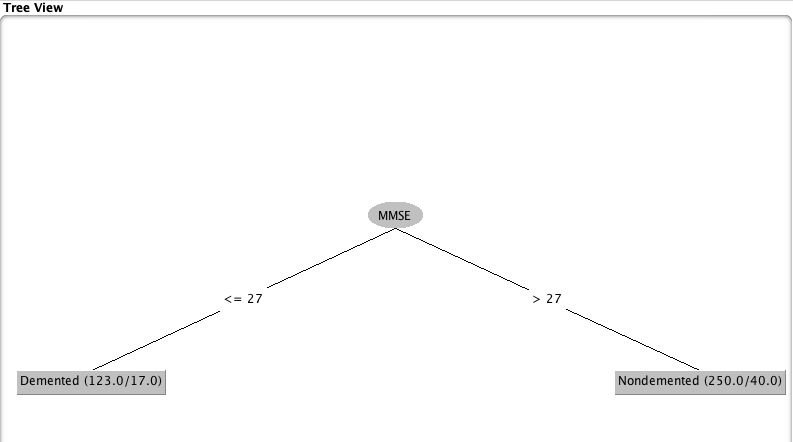
\includegraphics[width=1\linewidth]{J48Tree} The J48 model only uses the
mmse score to make a decision for the classification of the dementia
status of a patient. Because of its simplicity and high accuracy score
and low false negative rate i will pick this model

Last thing to do is to look at the ROC curve if the algorithm covers
most of the data.

\begin{Shaded}
\begin{Highlighting}[]
\CommentTok{\#install.packages("pROC")}
\FunctionTok{library}\NormalTok{(pROC)}

\NormalTok{RocDataNonDem }\OtherTok{\textless{}{-}} \FunctionTok{read.arff}\NormalTok{(}\AttributeTok{file =} \StringTok{\textquotesingle{}RocDataNondem.arff\textquotesingle{}}\NormalTok{)}
\NormalTok{RocDataNonDemTrainSet }\OtherTok{\textless{}{-}} \FunctionTok{read.arff}\NormalTok{(}\AttributeTok{file =} \StringTok{\textquotesingle{}RocDataNonDemTrainSet.arff\textquotesingle{}}\NormalTok{)}

\NormalTok{colors }\OtherTok{\textless{}{-}} \FunctionTok{c}\NormalTok{(}\StringTok{"Cross{-}validation AUC: 0.793"} \OtherTok{=} \StringTok{"blue"}\NormalTok{, }\StringTok{"Training{-}set AUC: 0.827"} \OtherTok{=} \StringTok{"red"}\NormalTok{)}

\NormalTok{p }\OtherTok{\textless{}{-}} \FunctionTok{ggplot}\NormalTok{(RocDataNonDem, }\FunctionTok{aes}\NormalTok{(}\AttributeTok{x =} \StringTok{\textasciigrave{}}\AttributeTok{False Positive Rate}\StringTok{\textasciigrave{}}\NormalTok{, }\AttributeTok{y =} \StringTok{\textasciigrave{}}\AttributeTok{True Positive Rate}\StringTok{\textasciigrave{}}\NormalTok{)) }\SpecialCharTok{+} \FunctionTok{geom\_point}\NormalTok{() }\SpecialCharTok{+} \FunctionTok{geom\_point}\NormalTok{(}\AttributeTok{data =}\NormalTok{ RocDataNonDemTrainSet) }\SpecialCharTok{+} \FunctionTok{geom\_line}\NormalTok{(}\FunctionTok{aes}\NormalTok{(}\AttributeTok{color =} \StringTok{"Cross{-}validation AUC: 0.793"}\NormalTok{)) }\SpecialCharTok{+} \FunctionTok{geom\_line}\NormalTok{(}\AttributeTok{data =}\NormalTok{ RocDataNonDemTrainSet, }\FunctionTok{aes}\NormalTok{(}\AttributeTok{color =} \StringTok{"Training{-}set AUC: 0.827"}\NormalTok{)) }\SpecialCharTok{+}
  \FunctionTok{labs}\NormalTok{(}\AttributeTok{color =} \StringTok{\textquotesingle{}Legend\textquotesingle{}}\NormalTok{) }\SpecialCharTok{+} \FunctionTok{scale\_color\_manual}\NormalTok{(}\AttributeTok{values =}\NormalTok{ colors)}
\NormalTok{p }\OtherTok{\textless{}{-}}\NormalTok{ p }\SpecialCharTok{+} \FunctionTok{coord\_fixed}\NormalTok{()}
\NormalTok{p }\SpecialCharTok{+} \FunctionTok{ggtitle}\NormalTok{(}\StringTok{"Plot of Roc curve of J48 model"}\NormalTok{)}
\end{Highlighting}
\end{Shaded}

\includegraphics{Thema09DementiaPrediction_files/figure-latex/unnamed-chunk-27-1.pdf}
The above ROC plot illustrates the performance of the J48 algorithm,
evaluated through cross-validation and with the training set. A positive
aspect is that the ROC scores of the two lines are closely aligned,
indicating minimal overfitting. Although the score doesn't reach
perfection (1), the J48 algorithm emerges as the highest-scoring
algorithm for this dataset.

\#referenties

\url{https://meetinstrumentenzorg.nl/instrumenten/mini-mental-state-examination-gestandaardiseerde-versie/}

\end{document}
